%%
%% memoria.tex
%% 
%\documentclass[a4paper,12pt,titlepage,halfparskip, cleardoubleempty]{scrbook}
\documentclass[a4paper,12pt]{scrbook}
\pagestyle{headings}

% Referencias externas
\usepackage{xr-hyper}

%\usepackage[pdftex, breaklinks=false]{hyperref}
\usepackage[pdftex, breaklinks=false, colorlinks=true, linkcolor=black, anchorcolor=black, urlcolor=blue, citecolor=red]{hyperref}

%\usepackage[T1]{fontenc}
\usepackage[spanish]{babel}
\usepackage[utf8]{inputenc}

\usepackage[printonlyused]{acronym-custom}

\usepackage{inconsolata}

%\usepackage{titlesec}



%%%%%%%%%%%%%%%
% Paquetes para fuentes

% Paquete para la fuente charter
\usepackage{charter}

% Paquete para la fuente helvética
\usepackage[scaled=0.92]{helvet}

% Paquete para la fuente Courier
% \usepackage{courier}

% Guiones de hyphenado
\usepackage{hyphenat}

% Paquete para hacer un índice
\usepackage{makeidx}

% Extra ToC listings
\usepackage{tocbibind}

% Gráficos
\usepackage{graphicx}

% Extensión para el entorno enumerate ¿?
%\usepackage{enumerate}

% Paquete para cosas rotatorias ¿?¿?
%\usepackage{rotating}

% Paquete de matemáticas
%\usepackage{amstext}

% Define el entorno altt, como un verbatim pero se pueden utilizar fórmulas matemáticas
%\usepackage{alltt}

% Listados de código
%\usepackage{listings}

% Herramientas para alinear las comas decimales en columnas en un entorno tabular o array
%\usepackage{dcolumn}
%\usepackage{array}

% Extensión para el entorno tabular
%\usepackage{tabularx}

% Entornos wrapfigure y wraptable para poner texto alrededor de figuras
%\usepackage{wrapfig}

% Inclusión de pequeñas figuras ¿?¿?¿
%\usepackage{subfigure}

% Automatiza el resaltado de sintaxis usando pygments
\usepackage{minted}

\makeindex

\begin{document}

\input{ordenes.tex}

% Portada
\begin{titlepage}
  \centering
  \includegraphics[width=.3\textwidth]{logo_uca}

  \bigskip
  \bigskip
  \bigskip
  
%  \begin{changemargin}{3em}{3em}
    \centering

    {\Huge \textsc{\nohyphens{Escuela Superior de Ingeniería}}}
    
    \bigskip
    \bigskip
    \bigskip

    {\huge \nohyphens{Ingeniería Técnica en Informática de Sistemas}}

    \bigskip
    \bigskip
    \bigskip
    \bigskip
    \bigskip
    \bigskip

    {\LARGE \nohyphens{oFlute}}

    \bigskip
    \bigskip
    \bigskip
    \bigskip

    {\large Curso 2009-2010}

    \bigskip
    \bigskip
    \bigskip
    \bigskip
    \bigskip
    \bigskip
    \bigskip
      
%  \end{changemargin}

  {\Large José Tomás Tocino García \\}
  {\large Cádiz, \today}

\end{titlepage}

\cleardoublepage

% Segunda portada ¿?¿?
{
  \thispagestyle{empty}
  \centering
  \includegraphics[width=.2\textwidth]{logo_uca}

  \bigskip
  \bigskip
  \bigskip
  
  \begin{changemargin}{3em}{3em}

    \begin{center}
      {\Huge \textsc{\nohyphens{Escuela Superior de Ingeniería}}}
      
      \bigskip
      \bigskip
      
      {\huge \nohyphens{Ingeniería Técnica en Informática de Sistemas}}
      
      \bigskip
      \bigskip
      \bigskip
      \bigskip
      
      {\LARGE \nohyphens{\nombreProyecto}}

\marginpar{Añadir nombre completo}
      
      \bigskip
      \bigskip
      \bigskip
      \bigskip
      
    \end{center}
  \end{changemargin}
  \begin{changemargin}{3em}{1em}
  \begin{flushleft}
    \Large

    \textsc{Departamento}: \nohyphens{Lenguajes y Sistemas Informáticos.} \\
    \textsc{Director del proyecto}: \nohyphens{Manuel Palomo Duarte.} \\
    \textsc{Autor del Proyecto}: \nohyphens{José Tomás Tocino García}. \\
  \end{flushleft}

  \end{changemargin}  

  \bigskip
  \bigskip
  \bigskip
  
  \begin{flushright}
    \large
    Cádiz, \today

    \bigskip
    \bigskip
    \bigskip
    \bigskip    
    \bigskip
    \bigskip

    Fdo.: José Tomás Tocino García
    
  \end{flushright}

}


\cleardoublepage
\bigskip
\bigskip

Este documento se halla bajo la licencia \ac{FDL}. Según estipula la
licencia, se muestra aquí el aviso de copyright. Se ha usado la
versión inglesa de la licencia, al ser la única reconocida
oficialmente por la \ac{FSF}.

\begin{quote}
  Copyright \copyright  2010 José Tomás Tocino García.
  
  Permission is granted to copy, distribute and/or modify this document
  under the terms of the GNU Free Documentation License, Version 1.2
  or any later version published by the Free Software Foundation;
  with no Invariant Sections, no Front-Cover Texts, and no Back-Cover Texts.
  A copy of the license is included in the section entitled "GNU
  Free Documentation License".
\end{quote}

\cleardoublepage

\section*{Agradecimientos}

A Julian Raschke por crear y mantener Gosu.

\cleardoublepage

\tableofcontents
\listoffigures
\listoftables

\setlength{\parskip}{1.2ex plus 0.4ex minus 0.1ex}

\chapter{Introducción}
\section{nosequé nosécuanto}
blablabla introducción teórica mínima

\section{Objetivos}

Este proyecto blablabla

Los objetivos a cumplir son los siguientes

\section{Alcance}

El proyecto se compone de tres productos blablabla

\subsection{Limitaciones del proyecto}

Por limitaciones de tiempo blablabla

\subsection{Licencia}

El proyecto tiene licencia tal. Los componentes tienen las siguientes licencias:

\section{Glosario}

\subsection{Acrónimos}

\input{1.introduc/acronimos.tex}

\subsection{Definiciones}

\begin{description}
\item[Elemento definido] 
  \index{elemento}
  Definición
\end{description}

%Para poder enfrentarnos con garantías al desarrollo del proyecto es
necesario conocer una serie de conceptos relacionados con el sonido y
la música en general, y conceptos sobre análisis de señales que
explicaremos a lo largo de este capítulo.

\section{El sonido}
Un \textbf{sonido} es una vibración que se propaga por un medio
elástico en forma de onda. Estas vibraciones se transmiten de forma
longitudinal, esto es, en la misma dirección en la que se propaga el
sonido. El medio más común para la transmisión del sonido es el
\textbf{aire}. 

El sonido, en su forma más simple, se compone de una sola onda
sinusoidal básica, con las características tradicionales: amplitud,
frecuencia y fase.

\subsection{Frecuencia y tono}
La \textbf{frecuencia} mide el número de oscilaciones de la onda por
unidad de tiempo. Por regla general, se utiliza el \textbf{hercio}
como unidad de medida de frecuencia, que indica la cantidad de
repeticiones por segundo. La frecuencia determinará la \textbf{altura}
del sonido, es decir, cómo de grave o agudo es. Los sonidos graves
tienen una frecuencia baja, mientras que los sonidos agudos tienen una
frecuencia alta.

A lo largo de los años se ha establecido un estándar de referencia que
establece que la nota \textit{la} que se encuentra encima del
\textit{do} central del piano debe sonar a 440 hercios de
frecuencia. Esta medida se utiliza a la hora de afinar los
instrumentos, de modo que si al tocar la nota \textit{la} se detecta
un tono con una frecuencia de 440 hercios, entonces el instrumento
estará bien afinado.

El oído humano es capaz de detectar sonidos a partir de los 20
hercios. Los sonidos por debajo de esa frecuencia se conocen como
\textbf{infrasonidos}. Por otro lado, el límite auditivo en
frecuencias altas varía mucho con la edad: un adolescente puede oir
sonidos con frecuencias hasta los 18kHz, mientras que un adulto de
edad media solo suele llegar a captar sonidos de hasta 13kHz. El
límite genérico superior se establece en 20kHz, por encima de los
cuales los sonidos se denominan \textbf{ultrasonidos}.

\subsection{Amplitud}
La \textbf{amplitud} representa la energía que transporta la
onda. Cuando un instrumento u otro objeto genera una vibración, la
amplitud es la cantidad de movimiento que esa vibración genera.
Podría equipararse (de forma no estricta) a la intensidad del sonido:
cuanto mayor sea la amplitud, más fuerte se oirá el sonido.

\subsection{Fase}
Por último, la \textbf{fase} ($\varphi$) indica el desplazamiento
horizontal de la onda respecto del origen. Si la fase de una onda no
es cero, entonces parecerá que está \textit{desplazada} hacia la
derecha, si la fase es positiva, y hacia la izquierda si la fase es
negativa.

\begin{center}
  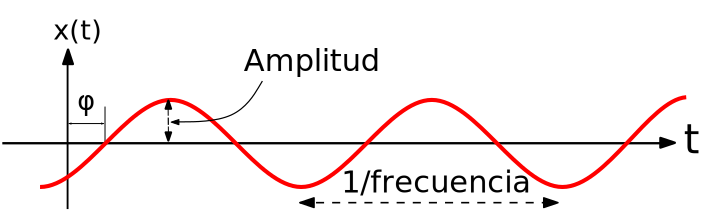
\includegraphics[scale=0.7]{conceptos/onda}  
\end{center}

\section{Descomponiendo sonidos}
Para desarrollar oFlute nos interesa conocer la altura de la nota que
está tocando la flauta en un instante concreto. Para un tono puro,
podríamos conocer la altura fijándonos en su frecuencia. El problema
es que, en la naturaleza, \textbf{no existen} los tonos puros, sino
que los sonidos se componen de multitud de tonos de diferentes
amplitudes, frecuencias y fases. 

Afortunadamente, la teoría dicta que cualquier onda periódica puede
descomponerse como suma de tonos puros de distintas frecuencias,
llamados \textbf{armónicos}. La menor de todas estas frecuencias se
conoce como \textbf{frecuencia fundamental}, y todas las otras
frecuencias son múltiplos enteros de ella. La frecuencia fundamental
es la que dicta la altura \textit{general} del sonido -- general, ya
que aunque las frecuencias de los otros armónicos pueden corresponder
a otras notas, es la altura de la frecuencia fundamental la que mayor
relevancia tiene en el sonido.

El resto de armónicos que acompañan a la frecuencia fundamental sirven
para enriquecer el sonido y, sobre todo, determinar el \textbf{timbre
  musical} del origen del sonido: Dos instrumentos pueden estar
tocando la misma nota y emitir la misma frecuencia fundamental, pero
será el conjunto total de armónicos el que nos ayude a distinguir uno
de otro.

La herramienta fundamental a la hora de descomponer una señal
periódica como puede ser un sonido es el \textbf{análisis de Fourier}.





\chapter{Desarrollo del calendario}
El proyecto no se ha desarrollado siguiendo un calendario estricto,
dado que era imposible cuantificar el tiempo que tomaría el adquirir
las bases teóricas necesarias para poder afrontarlo con garantías. Su
desarrollo se ha compaginado con los estudios del último curso de
Ingeniería Técnica en Informática de Sistemas y las labores como
becario en la Oficina de Software Libre y Conocimiento Abierto de la
Universidad de Cádiz~\cite{osluca}.

\section{Iteraciones}

Para la realización del presente proyecto se ha utilizado un modelo de
desarrollo iterativo incremental. A continuación se detallan cada una
de las etapas por las que ha ido pasando el software, y se observará
como conforme se iba avanzando se añadían nuevas funcionalidades y se
pulían las existentes.

\section{Diagrama de Gantt}

\section{Porcentajes de esfuerzo}


 
%\chapter{Descripción general del proyecto}
%
\section{Perspectiva del producto}

\section{Funciones}

Lista de funciones

\section{Características de los usuarios}

\section{Restricciones generales}

\section{Suposiciones y dependencias}


\section{Requisitos para futuras versiones}








 
\chapter{Investigación preliminar}
\input{3_investigacion/texto_investigacion.tex}

\chapter{Análisis}
\input{4_analisis/texto_analisis.tex}

\chapter{Diseño}
En este capítulo se presentarán los detalles de diseño del proyecto, basándonos
en el análisis mostrado en el capítulo anterior. El modelo de clases de diseño
representado aquí es más fiel a la implementación final que el diagrama de
clases conceptuales, pero aún así hay detalles que no se han contemplado por ser
demasiado cercanos a los detalles de implementación.

También en el presente capítulo se detallarán las decisiones de diseño en
relación al aspecto visual de la aplicación, extendiéndonos en el proceso de
creación del logotipo del juego así como de la interfaz gráfica de usuario.

\section{Diagrama de clases de diseño}

Tras la fase de diseño, componían el sistema más de 40 clases, por lo que hemos
tenido que dividir los diagramas en varias partes, intentando seguir cierto
criterio a la hora de elegir qué clases formarán parte de cada división.

En todos los diagramas aparecen, en aras de mantener el contexto, las clases
básicas de la aplicación: \textit{Juego} y \textit{Estado}. Además, hay algunas
otras clases que también se repetirán entre diagramas por conveniencia.

\begin{itemize}
\item En el primer diagrama (figura~\ref{diagrama_clases_1}) aparecen las clases
  relacionadas con el \textit{menú principal}, clases de utilidades (logging y
  animación), y clases para representar elementos gráficos.
\item En el segundo diagrama (figura~\ref{diagrama_clases_2}) aparecen las
  clases relacionadas con el subsistema de análisis del audio, así como las
  secciones \textit{Analizador de Notas} y \textit{Calibrar micrófono}.
\item En el tercer diagrama (figura~\ref{diagrama_clases_2}) aparecen todas las
  clases relacionadas con la sección de \textit{Canciones}.
\item En el cuarto y último diagrama (figura~\ref{diagrama_clases_2}) aparecen
  las clases relacionadas con el motor de \textit{lecciones}.
\end{itemize}

\begin{figure}[htp!]
  \centering
  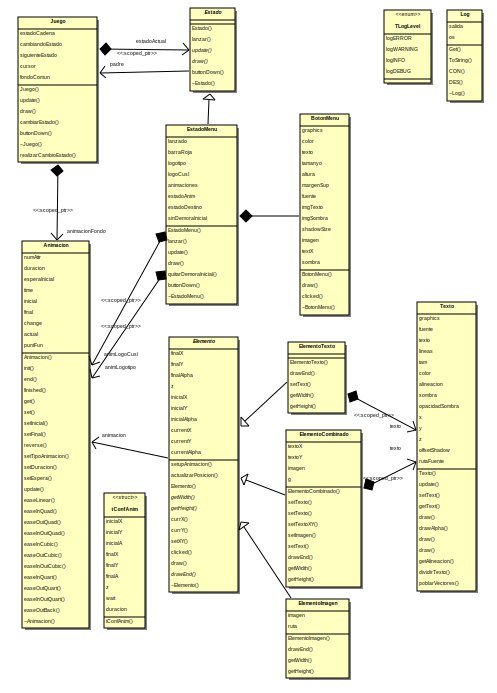
\includegraphics[width=\textwidth]{5_diseno/diagrama1}
  \caption{Diagrama de clases de diseño, parte I}
  \label{fig:diagrama_clases_1}
\end{figure}

\begin{figure}[htp!]
  \centering
  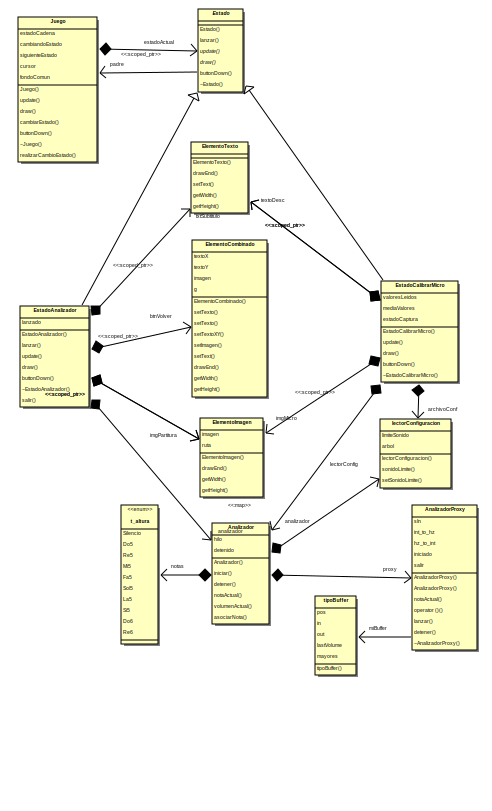
\includegraphics[width=\textwidth, clip=true, trim=0cm 3.5cm 0cm 0cm]{5_diseno/diagrama2}
  \caption{Diagrama de clases de diseño, parte II}
  \label{fig:diagrama_clases_2}
\end{figure}

\begin{figure}[htp!]
  \centering
  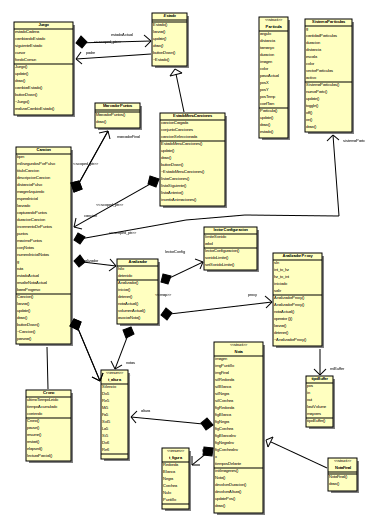
\includegraphics[width=\textwidth, clip=true, trim=0cm 0cm 0cm 0cm]{5_diseno/diagrama3}
  \caption{Diagrama de clases de diseño, parte III}
  \label{fig:diagrama_clases_3}
\end{figure}

\begin{figure}[htp!]
  \centering
  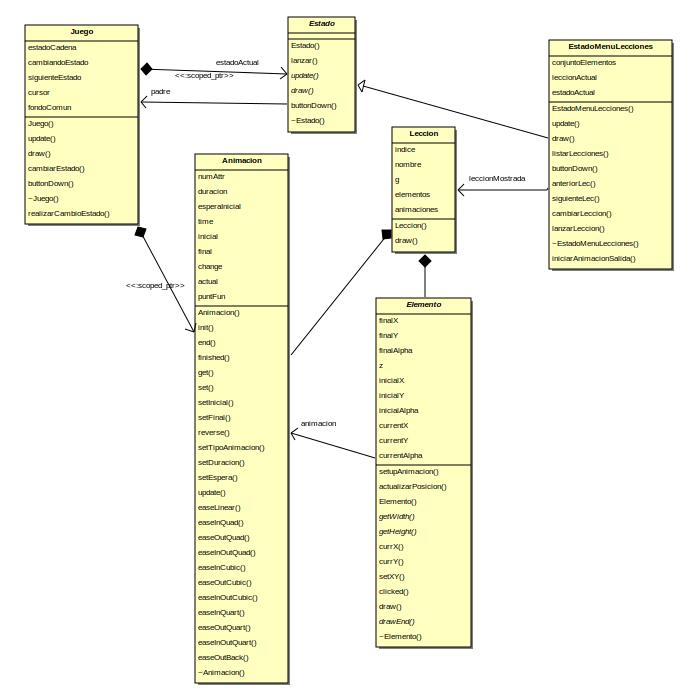
\includegraphics[width=\textwidth, clip=true, trim=0cm 0cm 0cm 0cm]{5_diseno/diagrama4}
  \caption{Diagrama de clases de diseño, parte IV}
  \label{fig:diagrama_clases_4}
\end{figure}

%%% Local Variables: 
%%% mode: latex
%%% TeX-master: "../memoria"
%%% End: 


\chapter{Implementación}
Un análisis claro y un diseño conciso no garantizan que, a la hora de
implementar el sistema planteado, no se encuentre ninguna dificultad o
imprevisto. Así pues, en este capítulo comentaremos los retos y detalles que más
relevancia o complejidad han presentado durante la fase de la implementación del
proyecto.

De igual modo, durante el desarrollo de la aplicacíon se mantuvo actualizada una
bitácora, accesible en línea~\cite{ofluteblog}, en la que se fueron detallando,
a medida que aparecían, muchas de estas dificultades.

Como complemento a la lectura de este capítulo se recomienda tener una copia
local del repositorio del proyecto, disponible para su libre descarga desde la
forja oficial~\cite{ofluteforja}. En él se encuentra todo el código fuente
original, así como la documentación en formato \textit{Doxygen}.

\section{Carga y uso de fuentes TrueType en Gosu}

Como se ha comentado previamente, \textbf{oFlute} hace uso de la biblioteca
\textit{Gosu}, que proporciona una API sencilla para el acceso al sistema
gráfico, entre otras características. Este framework funciona en sistemas
Windows, GNU/Linux y Mac OS, aunque dada la dificultad de conseguir la
compatibilidad con todos ellos, la calidad y el rendimiento es bastante
desigual de un sistema a otro.

Una de estas desigualdades se presentaba a la hora de \textbf{cargar fuentes}
para mostrar textos. En su versión para GNU/Linux, el módulo para el pintado de
textos de Gosu (que comprende la clase \texttt{Gosu::Font} y las funciones
\texttt{Gosu::drawText} y \texttt{Gosu::createText}) solo permitía
utilizar fuentes que estuvieran ya instaladas en el sistema de forma global, de
modo que era imposible adjuntar un fichero con una fuente en formato
\texttt{TrueType}~\cite{reftruetype} para su carga en el juego. 

La instalación de fuentes en sistemas GNU/Linux siempre ha sido una operación
engorrosa que ha requerido permisos de administrador. Esto, unido a que tanto en
Windows como en Mac OS la opción de cargar fuentes desde un fichero sí estaba
disponible, supuso un grave problema en el planteamiento del proyecto.

Inicialmente se investigaron las razones de esta limitación. Al ser un proyecto
libre y abierto, revisamos el código de Gosu, concretamente la implementación
de la clase \texttt{Gosu::Font} previamente citada, de la que dependían todas
las otras funciones relacionadas con fuentes.

Las conclusiones que se sacaron fueron que Gosu, bajo GNU/Linux, implementaba el
renderizado de fuentes mediante una biblioteca llamada Pango~\cite{Pango}, de
bastante bajo nivel, y que por diseño está limitada al uso de fuentes de
sistema, ya que se orienta a herramientas del sistema operativo, no a
aplicativos de terceros.

Así pues, era necesario buscar una alternativa. En numerosos proyectos
previos~\cite{robinson} se había utilizado la biblioteca
\textbf{SDL}~\cite{refsdl}, un framework multimedia muy utilizado en
aplicaciones de audio, vídeo y juegos. Uno de los subsistemas que proporciona
SDL es \textbf{SDL\_ttf}~\cite{refsdlttf}, una biblioteca para el renderizado de
fuentes basadas en ficheros \texttt{truetype}. Esto, unido a que la propia SDL
ya era una dependencia de Gosu, propició que se iniciara la implementación de
una solución basada en este medio.

\subsection{Funcionamiento de \texttt{SDL\_ttf}}

Para comprender cómo se implementó la solución al problema citado, el primer
paso es entender cómo funciona la biblioteca \texttt{SDL\_ttf} para poder ver
cómo se corresponde luego con Gosu.

\subsubsection{Tipos de datos utilizados}

En común con cualquier otra parte del conjunto de partes de SDL, SDL\_ttf se basa
en un tipo de datos conocido como \textit{superficies}
(\texttt{SDL\_Surface}). Estas superficies representan mapas de bits cargados en
memoria, y se utilizan para guardar las imágenes que se cargan de los ficheros,
así como para representar otros destinos gráficos intermedios, como la propia
pantalla.

Para representar el color del texto que vamos a pintar, SDL\_ttf utiliza la
estructura \texttt{SDL\_Color}, que guardará los valores de color de 8 bits para
cada uno de los canales.

Además, SDL\_ttf define un tipo de datos propio, de nombre \texttt{TTF\_Font}, que
representa una fuente cargada a partir de un fichero, con un tamaño determinado.

\subsubsection{Funciones utilizadas}

SDL\_ttf precisa de una \textbf{inicialización} previa, que se lleva a cabo mediante la
llamada a \texttt{TTF\_Init()}. Igualmente, liberaremos los recursos ocupados
mediante \texttt{TTF\_Quit()}.

Para \textbf{cargar la fuente} a partir de los ficheros TrueType (con extensión
\texttt{.ttf}), se utiliza la función \texttt{TTF\_OpenFont(const char * fichero,
  int tamaño)}. Esta función recibe una cadena con el nombre del fichero y el
tamaño de letra a utilizar, y devuelve un puntero al tipo \texttt{TTF\_Font}.

\begin{minted}{cpp}
  TTF_Font * fuente = TTF_OpenFont("fichero_fuente.ttf", 25);
\end{minted}

Una vez cargada la fuente de nuestro interés, tendremos que \textbf{generar una
  superficie} con el texto que queramos. Para ello, SDL\_ttf ofrece una gran
variedad de funciones, según el suavizado del texto y el tipo de caracteres que
estemos utilizando. En nuestro caso, queríamos que la superficie tuviera fondo
transparente, así como usar caracteres en UTF-8\cite{refutf8}, por lo que la
función que se eligió fue 
\begin{minted}{cpp}
  SDL_Surface * TTF_RenderUTF8_Blended (TTF_Font * fuente,
                                        const char * texto,
                                        SDL_Color color);
\end{minted}

Esta función devolverá un puntero a una superficie que se integrará
(\textit{blends}) sobre cualquier imagen, al tener el fondo transparente.


\subsection{Representación de imágenes en Gosu}

Una vez conocidos los tipos de datos y funciones que ofrece SDL\_ttf, es
necesario conocer cuáles son los tipos de datos equivalentes en Gosu, de forma
que pueda haber una \textit{conversión} de un tipo a otro.

\subsubsection{Mapas de bits de bajo nivel: Gosu::Bitmap}
La clase \texttt{Gosu::Bitmap} representa, en Gosu, un mapa de bits de bajo
nivel. Éste no contará con aceleración por hardware ni podrá mostrarse en
pantalla, pero podremos acceder directamente a los datos de los píxeles y
trabajar con ellos.

\texttt{Gosu::Bitmap} nos servirá de paso intermedio entre la superficie de SDL y las
imágenes habituales de Gosu.

\subsubsection{Imágenes de uso común: Gosu::Image}
En Gosu las imágenes y assets gráficos se manejan habitualmente con la clase
\texttt{Gosu::Image}, que representa un contenedor de más alto nivel que
\texttt{Gosu::Bitmap}, además de estar optimizado y poder pintarse en pantalla.

Podremos crear un objeto de esta clase a partir de un \texttt{Gosu::Bitmap}, consiguiendo
finalmente un objeto \textit{pintable}.


\subsection{Implementación final}

Conocidas las representaciones internas de ambas bibliotecas, la implementación
final fue una clase con una interfaz similar a \texttt{Gosu::Font}, de modo que
la transición pudiera ser lo más transparente posible, de nombre
\texttt{CustomFont}.

En el constructor de la se inicializa (de forma única, mediante una variable
estática) el subsistema \texttt{SDL\_ttf} utilizando la llamada
\texttt{TTF\_Init()}. Después, se carga la fuente indicada por los parámetros
del constructor. En ambos casos, se comprueba que el procedimiento ha sido
correcto, lanzando una excepción en caso contrario.

\begin{minted}{cpp}
static int initResult = TTF_Init();
if (initResult < 0)
   throw std::runtime_error("Could not initialize SDL_TTF");

font = TTF_OpenFont(fontName, fontHeight);
if (!font)
   throw std::runtime_error("Could not open TTF file " + fontName);

\end{minted}

Seguidamente, en el método de pintado (\texttt{draw}) se genera la superficie
con el texto que se indique, pasando el contenido de los píxeles a un contenedor
\texttt{Gosu::Bitmap} y finalmente generando un objeto \texttt{Gosu::Image} a
partir del mismo.

\begin{minted}{cpp}
SDL_Surface * surf = TTF_RenderUTF8_Blended(font, text, color);
if (!surface)
   throw std::runtime_error("Could not generate the surface");

Gosu::Bitmap temp;
temp.resize(surf.width(), surf.height());
std::memcpy(temp.data(), surf.data(), temp.width() * temp.height() * 4);

Gosu::Image image (graphic_target, temp);
image.draw(x, y, z);
\end{minted}

\subsection{Recepción}

Una vez contamos con una implementación funcional de la clase, se presentó el
parche en el foro oficial de Gosu~\cite{foroGosu}. En poco tiempo, el
desarrollador principal verificó el código propuesto e hizo una adaptación al
propio código original de la clase \texttt{Gosu::Font} para añadir la
propuesta. 

Por ende, desde la versión \textbf{RELLÉNAME}, el \textit{parche} forma parte
oficial de Gosu, y así se hace indicar en el fichero \texttt{TextUnix.cpp} de la
distribución oficial:

\begin{minted}{cpp}
// [...]

// Used for custom TTF files
// Adapted from customFont class by Jose Tomas Tocino Garcia (TheOm3ga)
class SDLTTFRenderer : boost::noncopyable

// [...]
\end{minted}

Así pues, dado que la solucíon propuesta se integró en la distribución oficial,
nos deshicimos de la clase \texttt{customFont} a favor de la actualización de
\texttt{Gosu::Font}, dado que al fin y al cabo el funcionamiento interno es
el mismo.

\section{Animaciones dinámicas}

Una de las decisiones iniciales de diseño fue la de hacer la interfaz gráfica de
usuario lo más atractiva posible, intentando utilizar gráficos amigables y, en
la medida de lo posible, animaciones y efectos dinámicos.

Con esto, se tornaba necesario crear un sistema de animaciones lo más versátil
posible, de forma que dotar a los elementos de la interfaz de movimiento fuera
un proceso sencillo. 

\subsection{Antecedentes: animaciones en Flash}
Para evitar reinventar la rueda y tener una base estable con la que empezar, se
investigaron sistemas de animaciones ya existentes, evaluando diferentes
enfoques y aproximaciones, sobre todo en sistemas altamente relacionados con las
animaciones. En particular, nos centramos en Adobe Flash (\textit{anteriormente
  Macromedia Flash}) y la gran cantidad de código disponible relacionado con la
generación de animaciones dinámicas.

Especialmente interesante es el trabajo de Robert Penner, un programador
americano muy interesado en la programación matemática, que ideó un sistema de
animaciones dinámicas para ActionScript~\cite{actionscript} 1.0 y 2.0. Penner,
en su libro \textit{Programming Macromedia Flash MX}~\cite{libropenner} incluyó
un capítulo llamado \textit{Motion, Tweening and Easing} (que dada su
popularidad acabó ofreciendo de forma gratuita~\cite{capitulopenner}), en el que
por primera vez presentó y explicó con detalle su sistema de animaciones.

En el citado capítulo se desgranan las animaciones como ecuaciones dependientes
del tiempo y de las posiciones inicial y final, de forma que fuera fácil generar
una serie de funciones para determinar la posición de un objeto en cada
instante. Una vez presentados los conceptos iniciales, Penner desvela una serie
de ecuaciones de movimiento (que acabaron siendo bautizadas y mundialmente
conocidas como las \textit{Penner's Easing Equations}). Estas ecuaciones modelan
un gran número de movimientos, en función de cómo varía la posición respecto del
tiempo (y perceptualmente la aceleración/deceleración del objeto animado).

Además, por cada tipo de ecuación, Robert Penner generó tres tipos de
movimientos: de aceleración (\textit{ease in}), de deceleración o frenada
(\textit{ease out}), y de aceleración-deceleración (\textit{ease in-out}). Con
esto, quedaban cubiertas la práctica totalidad de los tipos de animaciones posibles.

Así, un ejemplo de ecuación podrían ser las cúbicas, que hacen que la posición
del movimiento se rija por una función cúbica del tiempo. Si graficamos la
relación del tiempo por la posición, ambos de 0 a 1, el resultado sería el
siguiente:

{\Large\textbf{GRÁFICA x*x*x}}

Tras estudiar bien el código original, se decidió hacer una adaptación en C++,
de forma que se adaptara a las necesidades del proyecto.

\subsection{Adaptación en C++}
El primer paso fue portar las ecuaciones propiamente dichas -- esto es, las
funciones que generaban las posiciones intermedias. Dado que el lenguaje
original, ActionScript, es un derivado de EcmaScript~\cite{Ecmascript}, la
sintaxis es prácticamente idéntica a C++ en cuanto a asignaciones y operadores
se refiere, por lo que este paso fue prácticamente transparente.

Seguidamente, se ideó un \textit{wrapper} para estas ecuaciones, de forma que
fuera un objeto independiente el que se encargara de calcular las posiciones
intermedias de la animación, en lugar de tener que hacerlo los propios objetos
animados. Para ello, se creó la clase \texttt{Animación}, con las siguientes
características:
\begin{itemize}
\item Para cada instancia, permite animar un número arbitrario de valores, de
  forma que con un solo objeto \textit{Animacion} podamos animar la posición
  horizontal y vertical de un objeto, por ejemplo.
\item Permite elegir entre tres tipos de movimiento (\textit{ease in},
  \textit{ease out} y \textit{ease in-out}) para tres ecuaciones distintas
  (cuadrática, cúbica y cuártica), además de una ecuación especial con
  movimiento de ida y vuelta, y, lógicamente, movimiento uniforme. En total, 11
  posibles movimientos.
\item Capacidad para atrasar las animaciones, de forma que sea sencillo generar
  animaciones escalonadas de varios elementos sin tener que recurrir a
  \textit{callbacks}.
\end{itemize}

\subsection{Ejemplo de uso}

Supongamos que tenemos una pelota que queremos mover diagonalmente con un
movimiento de aceleración, desde la posición 0,0 hasta la posición 150, 300, en
30 pasos. Además, tenemos un cuadrado que habrá de moverse de la posición 0, 150
hasta la posición 150,150 cuando la pelota vaya por la mitad de su camino, y que
llegue a la vez que aquella.

Para cumplir este objetivo, crearemos dos objetos \texttt{Animación}, uno para
la pelota y otro para el cuadrado. En el caso de la pelota estaremos animando
dos parámetros, la posición horizontal y la vertical, y la duración será de 30
pasos. El tipo de movimiento será de aceleración, y la ecuación que elegiremos
será la cuadrática. Al no indicarse nada, no habrá espera inicial.

\begin{minted}{cpp}
// Creamos la instancia
Animacion animPelota (2, 30, Animacion::tEaseInQuad, 0);

// Asignamos la pos inicial y final de la coordenada horizontal
animPelota.set(0, 0, 150);  

// Coordenada vertical
animPelota.set(1, 0, 300);
\end{minted}

En el caso del cuadrado el movimiento sólo será horizontal, por lo que
animaremos un parámetro. Además, el movimiento comenzará cuando la anterior
animación vaya por la mitad (esto es, en el paso 15), y deberá llegar a la vez,
por lo que la duración será de 15 pasos.

\begin{minted}{cpp}
// Creamos la instancia de la clase
Animacion animCuadrado (1, 15, Animacion::tEaseInQuad, 15);

// Asignamos las posiciones inicial y final
animCuadrado.set(0, 0, 150);
\end{minted}

Una vez inicializados los objetos \texttt{Animación}, tendremos que hacer que,
en cada iteración del bucle de juego, las animaciones se actualicen. Para ello,
la clase \texttt{Animación} dispone de un método \texttt{update}. Además,
haremos uso del método \texttt{get} para obtener las posiciones intermedias y
así actualizar el objeto

\begin{minted}{cpp}
// ...
// En la fase update del bucle de juego
animPelota.update();
animCuadrado.update();

imagenPelota -> draw(animPelota.get(0), animPelota.get(1));
imagenCuadrado -> draw(animCuadrado.get(0), 150);
\end{minted}

Con esto, ya estará lista la animación de ambos objetos. De cualquier modo, la
clase \texttt{Animación} provee otros métodos que pueden resultar de interés,
como el método \texttt{finished}, que comprueba si las animaciones han
concluído. 

Además, las ecuaciones de los movimientos han sido implementadas en forma de
funciones estáticas, por lo que es posible acceder a las mismas para hacer
cálculos puntuales si fuera necesario. En tal caso, hay que tener en cuenta que
todas las ecuaciones reciben cuatro parámetros, estos son, en orden:

\begin{itemize}
\item Tiempo transcurrido.
\item Valor inicial del atributo a animar.
\item \textit{Delta} del atributo en la animación (final - inicial).
\item Duración de la animación en pasos.
\end{itemize}

Con esto, será posible controlar las animaciones de forma independiente, sin
necesidad de crear una instancia de la clase.



\chapter{Pruebas}

%\chapter{Resumen}
%\documentclass[a4paper,11pt]{article}

\usepackage{estiloBase}
\usepackage{colores}
\usepackage{bera}
\usepackage{comandos}


\def \titulo{oFlute: blablablá título largo}
\def \autor{Alumno: José Tomás Tocino García\\Tutores: Manuel Palomo Duarte, Antonio García Domínguez}
\def \fecha{Agosto de 2010}

%\margenes

% Directorio de imágenes
%\graphicspath{{../img/}}

\begin{document}
\portada

\abstract{\textbf{oFlute} se modela como una herramienta lúdico-educativa para
  alumnos que comiencen a aprender a usar la flauta dulce, proporcionando un
  entorno atractivo y ameno para el estudiante. Éstos tendrán la posibilidad de
  comprobar sus conocimientos sobre el uso de la flauta de forma totalmente
  práctica, gracias a un motor de análisis del sonido capaz de detectar las
  notas que emite el jugador con la flauta, capturadas por un micrófono,
  mediante el que la aplicación valorará la pericia del estudiante con la
  flauta.

  Además, los jugadores podrán recorrer una serie de pequeñas lecciones sobre
  música en general, y el uso de la flauta dulce en particular. Estas lecciones
  son totalmente ampliables, dando al usuario la posibilidad de crear las suyas
  propias. }

\vspace{0.5cm}

\begin{center}
{\footnotesize Este documento se halla bajo la licencia FDL de GNU (Free Documentation
  License)\\ \url{http://www.gnu.org/licenses/fdl.html} }   
\end{center}



\tableofcontents

\lstset{style=C++}

%\setlength{\parskip}{0.3cm plus 3mm}
\setlength{\parindent}{0.3cm}

\section{Introducción}

\subsection{Contexto y motivación}
Las nuevas tecnologías van filtrándose gradualmente en los centros
educativos, y las técnicas de enseñanza se están adaptando a las
opciones que ofrecen. El reparto de ordenadores portátiles a los
alumnos andaluces de 5º y 6º de primaria, dentro del marco de la
Escuela TIC 2.0, es buena muestra de ello. 

Por otro lado, las nuevas generaciones están en plena simbiosis con las
tecnologías de la información, cada vez más acostumbradas al empleo de
dispositivos electrónicos interactivos, y su uso ya les es prácticamente
instintivo. Por tanto, es beneficioso buscar nuevos métodos educativos que hagan
uso de las nuevas tecnologías.

En la búsqueda de materias educativas en las que aplicar el uso de las nuevas
tecnologías, la música, parte fundamental del programa curricular en la
educación primaria, ofrece una gran variedad de aspectos que podrían
desarrollarse utilizando tecnologías de la información. Es ahí donde este
proyecto hace su aportación, en la flauta dulce, un instrumento económico y
fácil de aprender que se usa tradicionalmente en la educación musical
obligatoria en España.

\subsection{Objetivos}
Los principales objetivos a alcanzar con \textbf{oFlute} son los siguientes:

\begin{itemize}
\item Crear un módulo de análisis del sonido en el dominio de la frecuencia para
  poder identificar las notas emitidas por una flauta dulce y capturadas
  mediante un micrófono en tiempo real.
\item Crear una aplicación de usuario que identifique y muestre en pantalla las
  notas que toca el usuario con la flauta dulce en cada momento.
\item Reutilizar el módulo de análisis en un juego en el que el
  usuario debe tocar correctamente las notas que aparecen en pantalla
  siguiendo un pentagrama.
\item Incluir un sistema de lecciones multimedia individuales que
  sirvan al alumno de referencia y fuente de aprendizaje.
\item Potenciar el uso de interfaces de usuario amigables, con un
  sistema avanzado de animaciones que proporcione un aspecto fluido y
  evite saltos bruscos entre secciones.
\item Obtener una base teórica sobre cómo se representa y caracteriza
  digitalmente el sonido.
\item Conocer las bases del DSP, y su uso en aplicaciones de
  reconocimiento básico de sonidos, tales como sintonizadores y
  afinadores de instrumentos.
\item Adquirir soltura en la programación de audio bajo sistemas GNU/Linux.
\item Entender las bases del análisis de sonidos en el dominio de la
  frecuencia. 
\item Utilizar un enfoque de análisis, diseño y codificación orientado
  a objetos, de una forma lo más clara y modular posible, para
  permitir ampliaciones y modificaciones sobre la aplicación por
  terceras personas.
\item Hacer uso de herramientas básicas en el desarrollo de software,
  como son los Sistemas de Control de Versiones para llevar
  un control realista del desarrollo del software, así como hacer de
  las veces de sistema de copias de seguridad.

\end{itemize}

\section{Planificación}

\section{Descripción general}

\section{Implementación}

\section{Conclusiones y difusión}



\end{document}

 
\chapter{Conclusiones}
%%%
%% Conclusiones del proyecto
%% Copyright (C) 2008 Antonio Garc�a Dom�nguez
%% $Id: conclusiones.tex 625 2008-07-03 14:46:36Z antonio $
%%

\section{Valoraci�n}

El trabajo realizado durante este PFC se puede considerar un ejemplo
de c�mo Extreme Programming permite, incluso con limitaciones de
tiempo, entregar un producto funcional y de calidad, limitando en la
medida necesaria el alcance.

El subconjunto de la salida de \ac{ACL2} sigue estando limitado a
casos de inter�s sobre todo did�ctico, pero se han superado las
primeras barreras frente a proyectos de inter�s cient�fico, con el
soporte para proyectos con m�ltiples ficheros y la separaci�n completa
del an�lisis de los documentos Lisp, las salidas de \ac{ACL2}, y la
producci�n del c�digo \ac{XML}.

Al mismo tiempo, se ha podido comprobar la generalidad obtenida en el
visor, ahora con identidad propia bajo el nombre de \visor{},
a�adi�ndole soporte no para un lenguaje concreto, sino para la familia
completa de lenguajes del metalenguaje \ac{YAML} 1.1 y su subconjunto
\ac{JSON}.

Todas las propiedades deseables conseguidas en el Proyecto sobre el
que se basa el presente se han mantenido e incluso reforzado:

\begin{itemize}
\item La extensibilidad no pasa solamente ya por nuevas formas de ver
  la salida de \ac{ACL2}, sino que se pueden a�adir nuevos formatos,
  integr�ndose con los editores y conversores que necesitemos. Todo
  sin tener que modificar una sola l�nea de \visor{}. Esto supone
  tambi�n una ampliaci�n de la capacidad de reutilizaci�n de la l�gica
  de \visor{}.

\item La transportabilidad entre m�ltiples sistemas operativos y
  microarquitecturas se mantiene, y ahora es mucho m�s f�cil instalar
  \visor{} y sus conversores, especialmente en Windows.

\item Se ha traducido la interfaz completa al ingl�s, y el c�digo
  tambi�n est� en proceso de traducci�n. El nuevo wiki de
  \visor{}~\cite{WikiXMLEye} permitir� localizar tambi�n f�cilmente
  toda la documentaci�n, y la forja~\cite{ForjaXMLEye} en RedIris
  recopilar� los informes de errores, peticiones de nueva
  funcionalidad y los ficheros relacionados.
\end{itemize}

\section{Mejoras y ampliaciones}

\subsection{Funcionalidad}

Se extender� el soporte de la salida de \ac{ACL2}, empezando por
tutoriales de mayor alcance como~\cite{recindacl2}, cuya salida es 4
veces m�s larga que la mayor tratada por este programa, y hace uso de
varias caracter�sticas a�n no filtradas, como macros Lisp.

En cuanto a \ac{YAML}, se a�adir�n hojas de usuario para formatos
derivados de inter�s, como los marcadores de Firefox 3, por
ejemplo. Habr� que ver si las limitaciones impuestas por el lenguaje
Perl sobre \yaxml{} realmente suponen una p�rdida de funcionalidad
importante o no.

En futuras versiones, \visor{} incluir� la capacidad de publicar las
demostraciones en formato de p�gina Web. Queda por determinar si se
har� a trav�s de ficheros est�ticos, o si se incrustar� un servidor
Web sencillo, como Jetty (\url{http://www.mortbay.org/jetty-6/}).

Habiendo traducido la interfaz y la documentaci�n al ingl�s, queda por
completar la traducci�n del c�digo en s�. Esto ser� m�s complicado en
\postprocesador{}, ya que no hay herramientas de refactorizaci�n para
Perl. El c�digo de \yaxml{} ya se encuentra completamente en ingl�s.

\subsection{Dise�o}

El dise�o de \visor{} ya no cambiar� en gran medida, pero continuar�
siendo refinado y pulido, al mismo tiempo que se implementan m�s
pruebas de unidad sobre los propios modelos de presentaci�n de los
documentos y los formularios principal y de formatos admitidos. 

La creaci�n de nuevas interfaces, como la interfaz Web, ayudar�n a
localizar nuevas v�as de mejora de las pruebas y del dise�o actual. Se
definir�n nuevos tipos de visualizaciones, basadas en tecnolog�as como
\ac{SVG} o JavaFX, y se integrar�n motores \ac{XHTML} m�s avanzados,
como el de los proyectos Lobo (\url{http://www.lobobrowser.org/}) o
Flying Saucer (\url{https://xhtmlrenderer.dev.java.net}).

Se investigar�n formas de definir alg�n tipo de pruebas de unidad
sobre las hojas de usuario \ac{XSLT}: una posibilidad es utilizar
asertos XPath, por ejemplo, que son lo bastante flexibles como para
asegurar comprobaciones potentes, y al mismo tiempo mucho m�s robustos
que comparar directamente el c�digo fuente con los resultados
esperados.

El dise�o general de los m�dulos ya sigue las mejores pr�cticas del
\ac{CPAN}, pero es posible que \postprocesador{} siga cambiando a una
escala considerable: el manejo de macros seguramente requerir� una
revisi�n importante del dise�o actual, con la posibilidad de
instrumentar el c�digo Lisp original para obtener m�s informaci�n.

\section{Otros aspectos de inter�s}

El empaquetado ha sido notablemente mejorado, pero a�n hay cosas por
hacer: mediante Launch4J se podr�an crear ejecutables para \visor{} en
Windows que detectaran la carencia de un \ac{JRE} y dirigieran al
usuario a la p�gina de descarga de Sun. De todas formas, existen
paquetes para las versiones m�s recientes de la distribuci�n GNU/Linux
Ubuntu y archivos comprimidos listos para usar, adem�s de las usuales
distribuciones de c�digo fuente.

Adem�s, ahora el Proyecto completo se puede ejecutar al 100\% sobre
software libre, gracias a los esfuerzos de los proyectos
OpenJDK~\cite{OpenJDK} e IcedTea~\cite{IcedTea} para crear una versi�n
completamente libre de \ac{J2SE} 5.0.

Se desean enviar los paquetes Debian de \visor{} y sus conversores al
repositorio de paquetes Debian, y \yaxml{} al \ac{CPAN}, para
facilitar su adopci�n por usuarios potenciales.

%%% Local Variables: 
%%% mode: latex
%%% TeX-master: "../memoria"
%%% End: 


%\chapter{Manual del usuario}
%%
% Generado autom�ticamente por las hojas de estilo XSLT
% Modificado posteriormente a mano
%
% Antonio Garc�a Dom�nguez, (C) 2008
% nyoescape@gmail.com
% $Id$
%

\section{Instalaci�n de XMLEye}
\label{instPrograma}

 En este apartado cubrir� la instalaci�n de XMLEye en sus diferentes formas, tanto a nivel de usuario local como a nivel de sistema. Para instalar los conversores asociados y sus hojas de usuario y descriptores de formato, referirse al apartado~\ref{instHojas} (p�gina~\pageref{instHojas}). 

\subsection{Requisitos previos}

 Se necesita tener instalado un entorno Java compatible con J2SE 5.0 o superior. Su instalaci�n se realiza autom�ticamente si utilizamos los paquetes Debian. 

\subsubsection{Windows}

 Tendremos que ir a \url{http://java.sun.com/javase/downloads/index.jsp} y descargar una edici�n reciente del JRE de acuerdo a nuestro sistema operativo. Tanto si hemos obtenido la versi�n que no requiere conexi�n como la que descarga s�lo lo necesario a trav�s de Internet, todo lo que tendremos que hacer es ejecutar el instalador y seguir las instrucciones. 

\subsubsection{GNU/Linux}

 Si utilizamos una distribuci�n basada en Debian, podemos probar a instalar los paquetes \filename{icedtea\hyp{}7\hyp{}jre} o \filename{openjdk\hyp{}6\hyp{}jre}. OpenJDK es la iniciativa de Sun, que a fecha de hoy (03/07/2008) es pr�cticamente 100 \% libre salvo por algunas peque�as partes que el proyecto IcedTea ha reemplazado utilizando c�digo del proyecto GNU Classpath. Podemos instalar una versi�n de OpenJDK 6.0 con los reemplazos de IcedTea en Ubuntu 8.04 "Hardy Heron" y usarla como entorno Java por defecto con estas �rdenes: 

\begin{alltt}
	\command{sudo aptitude install openjdk-6-jre}
	\command{sudo update-alternatives --config java}
\end{alltt}

 Escogeremos la entrada de \filename{openjdk\hyp{}6\hyp{}jre} y pulsaremos Intro, terminando con este paso. Si estamos utilizando openSUSE 10.3, podemos usar sin problemas el entorno J2SE 5.0 de Sun que incluye de f�brica. En caso de que no estuviera instalado por alguna raz�n, tendr�amos que instalar los paquetes \filename{java\hyp{}1\_5\_0\hyp{}sun*} a trav�s del gestor de paquetes de YaST. 

\note{ Actualmente, OpenJDK sigue teniendo peque�os defectos en la forma en que sit�a los componentes Swing. Es posible que algunos di�logos tengan un aspecto distinto al normal, con botones demasiado grandes, por ejemplo. El JRE original de Sun no tiene estos problemas, pero no es 100 \% libre. De todas formas, los efectos de este problema son puramente est�ticos. }

\subsection{Instalaci�n desde distribuciones precompiladas}

\note{ Si se usa una distribuci�n basada en Debian, se deber�a considerar el uso de los paquetes Debian, que son mucho m�s c�modos de usar. }

\subsubsection{Un �nico usuario, GNU/Linux}

 El proceso es muy sencillo: s�lo hay que descargar el \filename{\hyp{}dist\hyp{}tar.gz} m�s reciente de XMLEye de \url{https://forja.rediris.es/frs/?group_id=233} y descomprimirlo bajo nuestro directorio personal. Para ejecutar XMLEye, basta con ejecutar el gui�n \filename{/home/\-\emph{usuario}/\-xmleye/\-xmleye} tras pulsar la combinaci�n \keycombo{ALT + F2}. Una opci�n m�s c�moda para los habituales de la l�nea de �rdenes es a�adir la siguiente l�nea a \filename{\~\{\}/\-.bashrc}: 

\begin{alltt}
export PATH=\$PATH:\~{}/xmleye
\end{alltt}

 Haciendo esto, se puede abrir cualquier documento compatible desde la l�nea de �rdenes mediante: 

\begin{alltt}
xmleye \emph{(ruta absoluta o relativa)}
\end{alltt}

 Seg�n este procedimiento, las hojas de usuario se instalar�n en \filename{/home/\-\emph{usuario}/\-xmleye/\-xslt}, y los descriptores de formatos en \filename{/home/\-\emph{usuario}/\-xmleye/\-formats}. Las opciones se guardar�n en \filename{/home/\-\emph{usuario}/\-xmleye}. 

\subsubsection{M�ltiples usuarios, GNU/Linux}

 Un caso m�s complejo es cuando queremos instalarlo para varios usuarios, pero queremos tener ajustes distintos para cada usuario (las hojas son comunes a todos). Al igual que en el caso anterior, deberemos tener instalado un JRE compatible con J2SE 5.0 o superior antes que nada, pero despu�s usaremos una distribuci�n diferente de los ficheros. 

 La distribuci�n "ideal" ser�a la del paquete Debian, pero como es un poco m�s compleja de lo que necesitamos, nos limitaremos a un t�rmino medio. Primero descomprimiremos la �ltima distribuci�n de XMLEye (el enlace de descarga est� en la secci�n anterior) a \filename{/opt}, que crearemos si no existe ya: 

\begin{alltt}
sudo mkdir /opt
cd /opt
sudo tar xjf \emph{(ruta a distribuci�n)}

\end{alltt}

 Tendremos que retocar el gui�n de lanzamiento un poco. XMLEye cuenta con dos variables de entorno, \envar{XMLEYE\_PREF\_DIR} y \envar{XMLEYE\_FORMATS\_DIR}, que indican la ruta en la que se guardar�n las preferencias y los formatos personalizados por el usuario. Adem�s, XMLEye supone que las hojas de usuario se hallan bajo el subdirectorio \filename{xslt} de la ruta sobre la cual es lanzado. 

 Teniendo todo esto en cuenta, habr� que sustituir las l�neas que afectan a \envar{PROGRAM\_DIR} y \envar{PROGRAM\_JAR} por: 

\begin{alltt}
PROGRAM\_DIR=/opt/xmleye
PROGRAM\_JAR=xmleye.jar
export XMLEYE\_PREF\_DIR=\${HOME}/.xmleye
export XMLEYE\_FORMATS\_DIR=\${HOME}/.xmleye
mkdir -p \${XMLEYE\_PREF\_DIR}
\end{alltt}

 De forma similar a la secci�n anterior, los usuarios podr�an directamente ejecutar XMLEye a trav�s de la ruta completa. Para que todos los usuarios puedan ejecutar XMLEye por nombre, se puede a�adir esta l�nea a \filename{/etc/\-environment}: 

\begin{alltt}
export PATH=\$PATH:/opt/xmleye
\end{alltt}

 Si queremos que aparezca una entrada de men� y que se asocien los ficheros XML con XMLEye, entonces tendremos que, adem�s de seguir el paso anterior, crear el fichero \filename{/usr/\-share/\-applications/\-xmleye.desktop} con este contenido: 

\begin{alltt}
[Desktop Entry]
Encoding=UTF-8
Version=1.0
Type=Application
Terminal=false
Exec=xmleye  \%U
Comment[es]=Visor gen�rico de XML dirigido por datos
Name=XMLEye
Comment=Generic data-driven XML Viewer
GenericName=Generic XML viewer
GenericName[es]=Visor gen�rico de XML
Icon=accessories-text-editor
Categories=Utility;TextEditor;
MimeType=application/xml;
\end{alltt}

 Actualizaremos las bases de datos y reiniciaremos los men�s de GNOME con: 

\begin{alltt}
sudo update-desktop-database
sudo update-menus
sudo killall gnome-panel nautilus
\end{alltt}

 Ya deber�a de aparecer la entrada de XMLEye en el men� principal de GNOME. 

 Las hojas de usuario estar�n bajo \filename{/opt/\-xmleye/\-xslt}, y los descriptores de formato en \filename{/opt/\-xmleye/\-formats}. 

\subsubsection{Windows}

 Descargamos y descomprimimos en alguna carpeta el \filename{\hyp{}dist\hyp{}tar.gz} m�s reciente de XMLEye de \url{https://forja.rediris.es/frs/?group_id=233}. 

 Para ejecutar XMLEye, haremos doble clic en el fichero \filename{xmleye.jar} de la carpeta en que hemos descomprimido la distribuci�n. 

\subsection{Instalaci�n desde paquetes Debian}

 Esta es la opci�n a seguir siempre que sea posible, ya que adem�s de ser m�s sencilla, permitir� recibir actualizaciones de forma autom�tica. 

 Los paquetes han sido desarrollados para Ubuntu Gutsy, pero deber�an funcionar en cualquier distribuci�n basada en Debian reciente. 

 Los pasos a seguir son: 

\begin{enumerate}
\item Descargaremos la firma digital de los paquetes disponible bajo \url{http://www.shoyusauce.org/packages/claveDebian.asc}.

\item  A�adiremos la firma al anillo de confianza de Apt. En primer lugar lanzaremos la opci�n \emph{Sistema $\rightarrow$ Administraci�n $\rightarrow$ Or�genes
	  de software} bajo el men� principal de GNOME. 

 Hecho esto, seleccionaremos la pesta�a \guilabel[moreinfo = none]{Autentificaci�n} y pulsaremos en el bot�n \guibutton[moreinfo = none]{Importar clave...}, tras lo cual seleccionaremos la firma que antes descargamos. 

 A�n no cerraremos la ventana: nos queda una cosa por hacer. 

\item  Ahora a�adiremos los repositorios de paquetes binarios y paquetes de fuentes de \application{XMLEye} y sus hojas de estilos. Esta vez iremos a la pesta�a \guilabel[moreinfo = none]{Software de terceros}. 

 Pulsaremos en \guibutton[moreinfo = none]{A�adir} e introduciremos esta l�nea tal y como est�: 

\begin{alltt}
deb http://www.shoyusauce.org/packages/ubuntu/ gutsy main
\end{alltt}

 Volvemos a pulsar en \guibutton[moreinfo = none]{A�adir}, pero esta vez introducimos esta l�nea: 

\begin{alltt}
deb-src http://www.shoyusauce.org/packages/ubuntu/ gutsy main
\end{alltt}

 Ya podemos pulsar en \guibutton[moreinfo = none]{Cerrar} para cerrar este di�logo, y solicitar la actualizaci�n de nuestras listas de paquetes en el di�logo subsecuente pulsando en \guibutton[moreinfo = none]{Recargar}. Una vez haya terminado, estaremos listos para instalar \application{XMLEye} y otros paquetes de apoyo, como \application{pprocACL2}. 

\item  Lanzaremos \emph{Sistema $\rightarrow$ Administraci�n $\rightarrow$ Gestor
	  de paquetes Synaptic} y pulsaremos en el bot�n \guibutton[moreinfo = none]{Buscar} de la barra de herramientas. 

 Introduciendo "xmleye" en el campo de b�squeda obtendremos un �nico resultado en el que podremos hacer doble clic para marcar para su instalaci�n. Tambi�n podr�amos seleccionar otros paquetes con los conversores, descriptores y hojas de estilos espec�ficas de otros formatos, como "libacl2-procesador-perl" o "libyaxml-reverse-perl", de la misma forma. 

 Una vez todos los paquetes que deseamos instalar se hallen marcados, pulsaremos en \guibutton[moreinfo = none]{Aplicar} de la barra de herramientas para confirmar los cambios. 

\item  �Listo! Ya podemos lanzar XMLEye a trav�s de \emph{Aplicaciones $\rightarrow$ Accesorios $\rightarrow$ XMLEye} del men� principal de GNOME. 

\note{ S�lo un detalle: todas las opciones que establezcamos ir�n a parar al subdirectorio \filename{.xmleye} bajo nuestro directorio personal, es decir, \filename{/home/\-\emph{nombredeusuario}}. }

\end{enumerate}

 La ruta bajo la cual tendremos que instalar las hojas de usuario ser� \filename{/usr/\-share/\-xmleye/\-xslt}, y en \filename{/usr/\-share/\-xmleye/\-formats} se hallar�n los descriptores de formato. 

\subsection{Compilaci�n del c�digo fuente}

\note{ Aunque hay instant�neas disponibles del c�digo fuente, �stas son m�s para los usuarios que los desarrolladores. En caso de querer participar como desarrollador, recomiendo encarecidamente usar una copia de trabajo del repositorio Subversion. Bastar� con instalar el paquete \filename{subversion} y seguir algunas instrucciones sencillas. Para m�s informaci�n, v�ase el excelente libro~\cite{svnhandbook}. }

 Tras obtener un JDK compatible con J2SE 5.0 o superior, como el de OpenJDK 6.0 o 7.0, IcedTea 6.0 o 7.0, o los originales de Sun, tendremos que instalar adem�s la herramienta Apache Ant y el entorno de pruebas de unidad JUnit, en una de sus versiones 3.X. En Ubuntu 8.04 "Hardy Heron", esto se puede hacer mediante: 

\begin{alltt}
sudo aptitude install openjdk-6-jdk ant junit
\end{alltt}

 Ahora tendremos que crear una copia de trabajo local de la �ltima revisi�n de la rama principal de desarrollo del repositorio de RedIris: 

\begin{verbatim}
svn checkout \
  https://forja.rediris.es/svn/csl2-xmleye/XMLEye/trunk \
  xmleye
\end{verbatim}

 Ya podemos introducirnos en \filename{xmleye} y aprovechar los objetivos ya definidos en el fichero \filename{build.xml} de Ant. Si se desea instalar \filename{xmleye} a partir de fuentes, se recomienda usar el objetivo \varname{dist} e instalar la distribuci�n seg�n alguno de los m�todos antes expuestos. 

\begin{description}
\item[clean] \mbox{}
Limpia el �rbol de directorios existente.

\item[compile] \mbox{}
Compila todo el c�digo fuente.

\item[dist] \mbox{}
Compila las fuentes ,ejecuta las pruebas de unidad y genera una distribuci�n autocontenida en el subdirectorio \filename{dist}.

\item[dist-jar] \mbox{}
Tras compilar y ejecutar las pruebas de unidad, genera un fichero \filename{.jar} bajo \filename{dist}, pero no llega a empaquetarlo con todo lo dem�s.

\item[docs] \mbox{}
Genera la documentaci�n del API en formato HTML en el subdirectorio \filename{docs} a trav�s de Javadoc.

\item[run] \mbox{}
Se trata del objetivo por defecto (ejecutado a trav�s de \command{ant}). Compila el c�digo y ejecuta la versi�n as� compilada de XMLEye.

\item[run-about] \mbox{}
Compila el c�digo y ejecuta �nicamente la ventana de "Acerca de". �til a la hora de dise�ar la interfaz.

\item[run-find] \mbox{}
Como la anterior, pero para el di�logo de b�squeda.

\item[run-types] \mbox{}
M�s de lo mismo, pero para el di�logo de edici�n de tipos.

\item[test] \mbox{}
Ejecuta las pruebas de unidad. La salida de cada conjunto de pruebas se halla bajo el fichero \filename{TEST\hyp{}*} correspondiente.

\end{description}

 M�s cosas a tener en cuenta: esta aplicaci�n depende de InfoNode Tabbed Panel 1.5.0 (licenciado bajo la GPL para uso no comercial) y del look and feel JGoodies Looks 2.1.4 (licenciado bajo BSD), disponibles en \url{http://www.infonode.net/index.html?itp} y \url{https://looks.dev.java.net/} respectivamente. De todas formas, los ficheros \filename{.jar} necesarios se hallan en el propio repositorio, por lo que no hay que hacer nada al respecto. 

 Adem�s, el desarrollo puede hacerse mucho m�s c�modamente si se emplea el plugin Subclipse para Eclipse, disponible en \url{http://subclipse.tigris.org/}, y se importa a trav�s de �l el proyecto Eclipse desde el repositorio. As� podemos contar con sus funcionalidades de refactorizaci�n y notificaci�n de errores y avisos de compilaci�n en directo. 

\section{Instalaci�n de conversores asociados}

\label{instHojas}

\subsection{\nombrepostprocesador{}: convertidor de demostraciones de ACL2}

 Como muestra de las capacidades de XMLEye, desarroll� en paralelo un conjunto de hojas de usuario de preprocesado y visualizaci�n, junto con un tipo de documento para ACL2. Esto nos permite demostraciones para dicho sistema en formato \filename{.lisp} siguiendo una estructura arb�rea donde cada nodo se muestra como un hipertexto con enlaces a otras partes de la demostraci�n. 

 La subcarpeta \filename{t/\-testInputs} del fichero de fuentes con nombre de la forma \filename{ACL2\hyp{}Procesador\hyp{}*.tar.gz} m�s reciente contiene algunos ejemplos de inter�s, extra�dos de tutoriales reales de aprendizaje del uso de ACL2. 

 Primero nos ocuparemos de las dependencias, y luego veremos tres formas de instalar el convertidor, el descriptor de formato y las hojas de usuario. 

\subsubsection{Dependencias}

Las dependencias a instalar variar�n seg�n el m�todo de instalaci�n.

\paragraph{ACL2 2.9 o superior}

 Se ha depurado \postprocesador{} tambi�n con ACL2 3.1 y 3.3. 

\subparagraph{GNU/Linux}

En una distribuci�n basada en Debian, instalar ACL2 es tan sencillo como ejecutar la siguiente orden (necesitamos \application{gcc} para poder certificar libros):

\begin{alltt}
\command{sudo aptitude install acl2 gcc}
\end{alltt}

Otras distribuciones requerir�n del proceso manual de instalaci�n, documentado bajo \url{http://www.cs.utexas.edu/users/moore/acl2/v3-3/installation/installation.html}. Es sencillo, pero la compilaci�n de los libros puede llevar mucho tiempo (alrededor de 8-10 horas).

\subparagraph{Windows}

Descargaremos e instalaremos la distribuci�n completa de ACL2 preparada por Jared Davis, disponible en \url{http://www.cs.utexas.edu/users/moore/acl2/v3-3/distrib/windows/}. Incluye todo lo que podr�amos necesitar para trabajar con ACL2:

\begin{itemize}
\item ACL2 3.3

\item GCL 2.6.7, el entorno Lisp que necesitamos, junto con el compilador GCC necesario para certificar libros.

\item El editor GNU Emacs en su versi�n 21.3.

\item Documentaci�n de ACL2.

\item Una colecci�n de libros previamente certificados.

\end{itemize}

\paragraph{Perl 5.8.6 o superior}
\label{inst_perl}
\subparagraph{GNU/Linux}

 La gran mayor�a de las distribuciones lo incluyen de f�brica, pero en el caso en que no lo tuvi�ramos, podr�amos instalarlo en una distribuci�n basada en Debian con: 

\begin{alltt}
\command{sudo aptitude install perl}
\end{alltt}

Otra opci�n ser�a descargar el c�digo fuente de \url{http://www.perl.com/download.csp} y compilarlo, pero no se cubrir� dicha alternativa aqu�.

\subparagraph{Windows}

 Utilizaremos la edici�n 5.10 m�s reciente de Strawberry Perl, disponible bajo \url{http://strawberryperl.com/}. S�lo hemos de seguir los pasos del instalador. 

\paragraph{M�dulos Perl: \application{PAR}}
\label{inst_par}
 Una vez hayamos instalado Perl (v�ase la secci�n ), s�lo necesitamos ejecutar una orden m�s. No es necesario seguir la configuraci�n manual del acceso a CPAN en ninguno de los dos casos. 

\subparagraph{GNU/Linux}

\begin{alltt}
\command{sudo cpan PAR}
\end{alltt}

\subparagraph{Windows}

\begin{alltt}
\command{cpan PAR}
\end{alltt}

\paragraph{M�dulos Perl: \application{PAR::Packer}}
\label{inst_parpacker}
\subparagraph{GNU/Linux}

 Si estamos usando una distribuci�n basada en Debian reciente, podemos ejecutar: 

\begin{alltt}
\command{sudo aptitude install libpar-packer-perl}
\end{alltt}

 De lo contrario, ejecutaremos: 

\begin{alltt}
\command{sudo cpan PAR::Packer}
\end{alltt}

\subparagraph{Windows}

 Tendremos que obtener la �ltima copia del c�digo fuente de \application{PAR::Packer} del repositorio SVN, ya que la versi�n m�s reciente en el CPAN a d�a de hoy (03/07/2008), la 0.980, no incluye el arreglo de un defecto que imposibilitaba su instalaci�n en Strawberry Perl. Para ello, instalaremos el cliente Subversion TortoiseSVN, disponible bajo \url{http://tortoisesvn.tigris.org/}, y haremos un \emph{checkout} de la direcci�n \url{http://svn.openfoundry.org/par/PAR-Packer/trunk/}. 

 Una vez hayamos descargado el c�digo, abriremos una ventana del int�rprete de �rdenes, y dentro del directorio con el c�digo fuente, ejecutaremos: 

\begin{alltt}
\computeroutput{perl Makefile.PL
dmake
dmake test
dmake install
}
\end{alltt}

 Si se nos pide instalar alguna dependencia en alguno de los pasos, aceptaremos. 

\paragraph{Biblioteca \application{libxml2}}
\label{inst_xml}
\subparagraph{GNU/Linux}

 Si estamos usando una distribuci�n basada en Debian, ejecutaremos esta orden: 

\begin{alltt}
\command{sudo aptitude install libxml2-dev}
\end{alltt}

\subparagraph{Windows}

 No hay que hacer nada: viene ya incluida con Strawberry Perl. 

\subsubsection{Instalaci�n mediante paquetes Debian}

 Si instalamos XMLEye mediante el paquete Debian, s�lo tendremos que instalar el paquete \filename{libacl2\hyp{}procesador\hyp{}perl}. La pr�xima vez que iniciemos XMLEye tendremos todo lo necesario a nuestra disposici�n, incluido ACL2. 

\subsubsection{Instalaci�n desde distribuci�n monol�tica}
\label{inst_distrib_monolit}
 Necesitaremos previamente haber instalado ACL2, y haber instalado XMLEye descomprimiendo la distribuci�n de la forja. Descargaremos del �rea de ficheros (\url{http://forja.rediris.es/frs/?group_id=233}) de la forja de XMLEye el fichero \filename{ACL2\hyp{}Procesador\hyp{}*\hyp{}standalone\hyp{}*.tar.gz} m�s reciente que se corresponda con la microarquitectura de nuestra CPU y nuestro sistema operativo, y lo descomprimiremos sobre el directorio en el que instalamos XMLEye. 

\subsubsection{Instalaci�n desde distribuci�n basada en PAR}
\label{inst_distrib_par}
 Necesitaremos ACL2, Perl y el m�dulo PAR. El proceso es id�ntico al de~\ref{inst_distrib_monolit} (p�gina~\pageref{inst_distrib_monolit}), pero en este caso el fichero a descargar y descomprimir es \filename{ACL2\hyp{}Procesador\hyp{}*\hyp{}par\hyp{}noarch.tar.gz}, que es independiente de la CPU y el sistema operativo escogido. 

\subsubsection{Instalaci�n manual a partir de fuentes}
\label{inst_fuentes}
 Los pasos, tras instalar todas las dependencias, son los siguientes: 

\begin{enumerate}
\item Descomprimimos el fichero de fuentes bajo \filename{/tmp}, y nos introducimos en sus contenidos:

\begin{alltt}
cd /tmp
tar xzf \emph{(ruta a las fuentes)}
cd ACL2-Procesador-*
\end{alltt}

\item Instalamos el preprocesador tal y como instalar�amos cualquier paquete Perl. Este proceso resultar� muy familiar a cualquier usuario de las \application{autotools}:

\begin{alltt}
perl Makefile.PL
sudo make
make test
sudo make install
\end{alltt}

 Es muy probable que Perl nos solicite en la primera orden instalar algunas dependencias. Siempre le diremos que s�. La �ltima orden se podr�a sustituir por \command{sudo checkinstall} si deseamos poder desinstalarlo f�cilmente, instalando \postprocesador{} como un paquete Debian. 

\item  Lo siguiente es instalar las hojas de usuario, que es tan f�cil (suponiendo que la ruta de hojas de usuario es \filename{/home/\-\emph{tunombredeuaurio}/\-xmleye/\-xslt} como: 

\begin{alltt}
cp -r xslt/* \$HOME/xmleye/xslt
\end{alltt}

\item  Terminaremos instalando el descriptor de tipo a su sitio: 

\begin{alltt}
cp types/* \$HOME/xmleye/types
\end{alltt}

\end{enumerate}

\subsubsection{Ejecuci�n independiente de XMLEye}
\label{ejecucion}
 Podemos comproabr que todo va bien ejecutando el gui�n principal. La forma de hacerlo variar� seg�n el m�todo de instalaci�n usado: 

\begin{itemize}
\item Desde el paquete Debian, o desde fuentes: \command{pprocACL2} desde cualquier ruta.

\item Desde la distribuci�n monol�tica: \command{\emph{(ruta)}/\-pprocACL2}, utilizando la ruta bajo la cual se halla instalado XMLEye. Podr�amos a�adir esta ruta al PATH si quisi�ramos.

\item Desde la distribuci�n basada en PAR: \command{perl -MPAR (ruta)/\-pprocACL2.par}, utilizando la ruta bajo la cual se halla instalado XMLEye.

\end{itemize}

 Deber�amos obtener una salida como la que viene a continuaci�n. Por razones t�cnicas, es posible que en ciertos entornos la distribuci�n basada en PAR no produzca ninguna salida, pero esto no es un problema: seguir� funcionando de forma normal una vez le pasemos un fichero de entrada, imprimi�ndose el XML resultante por salida est�ndar, y los mensajes de estado por la salida de errores. 

\begin{alltt}
\computeroutput{Usage:
  pprocACL2 [opciones] [entrada Lisp ACL2]

Options:
  --help, -h, -?
          Se limita a mostrar un mensaje corto de ayuda.

  --man, -m
          Muestra un mensaje detallado de ayuda en formato man.}
\end{alltt}

\subsection{\nombreyaxml{}: conversor de documentos YAML a XML}

 Este otro conversor se desarroll� para abrir con XMLEye la familia completa de documentos con lenguajes basados en YAML 1.1 o JSON. Al igual que \postprocesador{}, incorpora las hojas de usuario y descriptores de formatos necesarios para su funcionamiento. Incluye soporte para anclias y alias de YAML. 

 Tambi�n en este caso se pueden ver algunos ejemplos de entradas aceptadas en \filename{t/\-testInputs} de las fuentes, disponibles como ficheros con nombres del estilo de \filename{YAXML\hyp{}Reverse\hyp{}*.tar.gz} en el �rea de ficheros de la forja (\url{http://forja.rediris.es/frs/?group_id=233}). 

 Para evitar repeticiones innecesarias, aprovecharemos las instrucciones de instalaci�n de algunas de las dependencias y algunos de los pasos de los m�todos de instalaci�n de \postprocesador{}. Comentaremos �nicamente los aspectos que cambian. 

\subsubsection{Dependencias}

Hay algunas dependencias de \application{YAXML::Reverse} cuyos m�todos
de instalaci�n ya se han mencionado en la secci�n \S\ref{inst_perl}
an�loga de \postprocesador{}:

\begin{description}
\item[Perl] \mbox{}
V�ase la p�gina~\pageref{inst_perl}.

\item[PAR] \mbox{}
V�ase la p�gina~\pageref{inst_par}.

\item[PAR::Packer] \mbox{}
V�ase la p�gina~\pageref{inst_parpacker}.

\item[Bibliotecas XML] \mbox{}
V�ase la p�gina~\pageref{inst_xml}.

\end{description}

\paragraph{Bibliotecas XSLT}

 Tambi�n puede que nos hagan falta las bibliotecas para XSLT. Dependiendo del sistema operativo sobre el que trabajemos, los m�todos de instalaci�n cambiar�n. 

\subparagraph{GNU/Linux}

 Necesitaremos instalar los paquetes de desarrollo para las bibliotecas \application{exslt}, \application{gdbm} y \application{gcrypt}. En una distribuci�n basada en Debian, usaremos: 

\begin{alltt}
\computeroutput{sudo aptitude install libexslt-dev \textbackslash{}
                      libgdbm-dev  \textbackslash{}
                      libgcrypt-dev}
\end{alltt}

\subparagraph{Windows}

 Como instalar manualmente las bibliotecas es demasiado complejo, usaremos una distribuci�n precompilada del m�dulo \application{XML::LibXSLT}. Para ello, ejecutaremos esta orden bajo la interfaz de l�nea de �rdenes: 

\begin{alltt}
\computeroutput{ppm install XML::LibXSLT}
\end{alltt}

\subsubsection{Instalaci�n mediante paquetes Debian}

Una vez instalemos XMLEye mediante el paquete Debian, s�lo habr� que instalar el paquete \filename{libyaxml\hyp{}reverse\hyp{}perl}, cerrar y volver a abrir XMLEye y todo quedar� listo.

\subsubsection{Instalaci�n desde distribuci�n monol�tica}

 En este caso utilizaremos el fichero m�s reciente que concuerde con nuestro entorno que siga el patr�n \filename{YAXML\hyp{}Reverse\hyp{}*\hyp{}standalone\hyp{}*.tar.gz}. 

\subsubsection{Instalaci�n desde distribuci�n basada en PAR}

 Esta vez las distribuciones (que siguen el patr�n \filename{YAXML\hyp{}Reverse\hyp{}*\hyp{}par\hyp{}*.tar.gz}) ser�n espec�ficas del entorno, pero por lo dem�s es todo igual. 

\subsubsection{Instalaci�n manual a partir de fuentes}

 El patr�n del nombre de fichero cambia a \filename{YAXML\hyp{}Reverse\hyp{}*.tar.gz} m�s reciente, y no se necesita ACL2, sino las bibliotecas de XSLT. El resto de las dependencias siguen siendo necesarias.

\subsubsection{Ejecuci�n independiente de XMLEye}

 El proceso es an�logo al de la secci�n~\ref{ejecucion} (p�gina~\pageref{ejecucion}), pero esta vez el gui�n principal es \filename{yaml2xml} (y el PAR es \filename{yaml2xml.par}), y la salida que deber�amos obtener tendr�a que ser similar a �sta: 

\begin{alltt}
\prompt{\$ yaml2xml}

\computeroutput{yaml2xml, using YAXML::Reverse 0.3.4
Usage: yaml2xml [path to .yaml]}
\end{alltt}

\subsection{Instrucciones gen�ricas}

 Estas instrucciones son las m�s detalladas, y sirven para cualquier hoja de usuario disponible actualmente y en el futuro, siempre que no var�e el dise�o de XMLEye. 

\subsubsection{Instalaci�n de hojas de usuario}

 Una hoja de usuario nos permite mejorar XMLEye en una de las siguientes formas: 

\begin{itemize}
\item Ver la estructura de un documento XML de otra forma. Un ejemplo ser�a ver s�lo un resumen del documento, cambiar el orden para su preprocesamiento, o decorar los nodos del �rbol con nuevas etiquetas e iconos.

\item Ver el contenido de un nodo del documento de otra forma. Podemos hacer cualquier cosa que se nos ocurra con XHTML 1.1 y CSS (no hay soporte para Javascript), y establecer v�nculos entre nodos del �rbol y nodos de otros documentos.

\end{itemize}

 Realmente, no son m�s que conjuntos de hojas XSLT que siguen una determinada estructura para permitir su localizaci�n y su integraci�n con otras hojas, ya que una hoja de usuario puede ser una especializaci�n de otra hoja. 

 La ruta donde se guardan las hojas de usuario variar� dependiendo del m�todo de instalaci�n que hayamos seguido. Para m�s detalles, referirse al apartado~\ref{instPrograma} (p�gina~\pageref{instPrograma}). Nos encontraremos bajo dicha ruta una serie de ficheros (s�lo de inter�s para desarrolladores) y dos subdirectorios, \filename{preproc} y \filename{view}, en cuyo interior habr� un subdirectorio por hoja de usuario de preprocesado o visualizaci�n, respectivamente. 

 Instalar una hoja de usuario no es m�s entonces que asegurarnos que su subdirectorio se halle en el lugar correcto, y reiniciar XMLEye. Encontraremos entradas con los mismo nombres que los subdirectorio correspondientes en las entradas \emph{Preferencias $\rightarrow$ Preprocesamiento} y \emph{Preferencias $\rightarrow$ Visualizaci�n} de XMLEye. Por defecto tendremos instalado como m�nimo las hojas de usuario de preprocesado y visualizaci�n \filename{xml}, y la hoja de visualizaci�n \filename{xmlSource} a partir de la versi�n 1.22. 

\subsubsection{Instalaci�n de nuevos formatos de documentos}

 A pesar de su nombre, XMLEye puede visualizar documentos de cualquier formato, usando un conversor si no se trata de un documento XML originalmente, e integrarse con su editor (monitorizando el fichero en busca de cambios) siempre que se le d� la informaci�n correspondiente. Esa informaci�n viene integrada en un \emph{descriptor de formato de documento}. 

 Dichos descriptores se nombran usando la extensi�n \filename{.format} y siguen un formato XML sencillo, en cuyos detalles no entraremos aqu� (v�ase el Manual del Desarrollador). Lo �nico que nos importa es su instalaci�n, que es tan sencilla como copiar el fichero \filename{.format} correspondiente a la ruta de tipos que le corresponde seg�n el tipo de instalaci�n que hayamos realizado. 

 Una vez instalado y reiniciado XMLEye, podremos abrir cualquier documento que tenga las extensiones especificadas en el tipo de documento instalado sin m�s problemas, siempre que su editor y preprocesador (si tiene alguno) se hallen debidamente instalados y tengan �rdenes que puedan ejecutarse desde el directorio principal de XMLEye (posiblemente usando ejecutables bajo los directorios dentro de la variable de entorno \envar{PATH}). 

\section{Uso y configuraci�n}
\label{uso}
Este apartado de la gu�a trata acerca del empleo de XMLEye y de su configuraci�n. Para cuestiones relacionadas con la instalaci�n o con detalles de implementaci�n, referirse a los apartados anteriores o al Manual del Desarrollador, respectivamente.

A lo largo de esta gu�a nos referiremos exclusivamente a las opciones de los men�s, pero pr�cticamente toda acci�n tiene una combinaci�n equivalente en el teclado,indicada en la parte derecha del elemento del men� correspondiente (y si no, es un fallo del que se agradecer�a una notificaci�n ;-): informe de �l en \url{https://forja.rediris.es/tracker/?group_id=233} ). Adem�s, las opciones m�s comunes poseen un bot�n en la barra de herramientas, cuyo icono es una versi�n ampliada del icono de la entrada de men� correspondiente.

Podemos cambiar entre los botones de la barra de herramientas, el �rbol y el navegador mediante \keycombo{Ctrl + Tab} en de izquierda a derecha y de arriba abajo, o mediante \keycombo{Shift + Ctrl + Tab} en direcci�n inversa.\keycombo{Tab} y \keycombo{Shift + Tab} siguen funcionando tambi�n de la forma usual, pero se hallan redefinidos en el navegador para navegar por los hiperv�nculos.

La forma de lanzar el programa se detalla en la gu�a de instalaci�n, y variar� seg�n el m�todo seguido.

\subsection{Apertura y edici�n de documentos}

 Bajo el men� \guimenu[moreinfo = none]{Fichero}, disponemos de \guimenuitem[moreinfo = none]{Abrir...}, en donde podremos seleccionar un fichero de cualquier tipo, o uno de los formatos que tengamos instalados. 

 Una vez hayamos seleccionado el fichero, XMLEye detectar� a partir de la extensi�n de qu� formato se trata y aplicar� el convertidor indicado, si lo hay. Una vez el fichero se halle disponible en formato XML, pasar� por la hoja de preprocesado y se mostrar� su �rbol en pantalla junto con la visualizaci�n de su nodo ra�z. 

 Para editar el fichero fuente con el editor definido en el descriptor de formato, usaremos \guimenuitem[moreinfo = none]{Editar fuente}. Si \emph{Preferencias $\rightarrow$ Actualizaci�n
      autom�tica} se halla activo, XMLEye monitorizar� el fichero en segundo plano y actualizar� el �rbol XML cada vez que se produzcan cambios en �l, indpendientemente de si estuviera o no el editor abierto. 

 Por �ltimo, podemos acceder a los 5 �ltimos documentos abiertos con �xito, o \guimenuitem[moreinfo = none]{Salir} del programa. 

 Para cerrar un documento, actualmente no hay ninguna entrada en el men� \guimenu[moreinfo = none]{Fichero}, pero puede hacerse pulsando la cruz de su pesta�a correspondiente. Para cerrar todos los documentos, podemos pulsar en el bot�n de cierre general en el extremo derecho del componente de pesta�as. 

\subsection{Navegaci�n por los documentos}

 El documento XML tras ser preprocesado sigue una estructura arb�rea normal y corriente, por lo que podemos realizar las acciones usuales mediante las entradas del men� \guimenu[moreinfo = none]{Navegar}. En particular: 

\begin{description}
\item[Buscar...] \mbox{}
 Abre un di�logo de b�squeda en el que podemos buscar siguiendo diversos par�metros. Adem�s de las opciones usuales de b�squeda por palabras completas o por concordancia de may�sculas, se puede marcar el �mbito de la b�squeda. 

\item[Buscar siguiente] \mbox{}
 Repite la �ltima b�squeda realizada, mostrando un error en caso de que no se halla realizado una anteriormente. Si hemos llegado al �ltimo resultado de la �ltima b�squeda, volveremos al primero despu�s. 

 La repetici�n de una b�squeda es muy r�pida, ya que XMLEye se ocupa de almacenar los resultados tras la primera petici�n y va dando directamente los resultados que le siguen dispu�s. 

\item[Padre] \mbox{}
 Sube un nivel en la jerarqu�a del �rbol, o no hace nada si estamos en la ra�z. 

\item[Hijo] \mbox{}
 Baja un nivel en la jerarqu�a del �rbol, o no hace nada si estamos en un nodo hoja. 

\item[Hermano anterior] \mbox{}
 Se desplaza al anterior nodo hijo del padre del nodo actual, o no hace nada si estamos en su primer hijo. 

\item[Hermano siguiente] \mbox{}
 Se desplaza al siguiente nodo hijo del padre del nodo actual, o no hace nada si estamos en su �ltimo hijo. 

\item[Expandir todo] \mbox{}
 Expande el contenido de todos los nodos del �rbol, de tal forma que todo nodo quede directamente visible, a menos que haya sido ocultado expl�citamente por la hoja de visualizaci�n. 

\item[Contraer todo] \mbox{}
 Contrae el contenido de todos los nodos del �rbol, de tal forma que �nicamente el nodo ra�z quede visible. 

\end{description}

Aunque casi toda acci�n es accesible mediante rat�n, se recomienda
aprender los accesos directos mediante teclado, ya que agilizan
enormemente los desplazamientos. En la tabla \ref{teclado_arbol}
(p�gina~\pageref{teclado_arbol}) se listan todos los accesos directos
mediante teclado para navegar por el �rbol del documento, tras hacer
clic en �l.

\begin{table}
\centering
\begin{tabularx}{\textwidth}{| c | X |} 
\hline
Combinaci�n de teclas & \multicolumn{1}{c|}{Efecto} \\ \hline
\hline
\keycombo{Arriba} & Selecciona el nodo anterior en la vista actual del �rbol. \\ \hline
\keycombo{Abajo} & Selecciona el nodo siguiente en la vista actual del �rbol. \\ \hline
\keycombo{Izquierda} & Sube al nodo padre si el nodo est� cerrado, y cierra el nodo actual de lo contrario. \\ \hline
\keycombo{Derecha} & Abre el nodo actual si est� cerrado, y baja al primer hijo de lo contrario. \\ \hline
\keycombo{Inicio} & Selecciona el primer nodo en la vista actual del �rbol. \\ \hline
\keycombo{Fin} & Selecciona el �ltimo nodo en la vista actual del �rbol. \\ \hline
\keycombo{Alt + Arriba} & Selecciona al nodo padre del actual. \\ \hline
\keycombo{Alt + Abajo} & Selecciona al primer hijo del nodo actual. \\ \hline
\keycombo{Alt + Izquierda} & Selecciona al hermano anterior del nodo actual. \\ \hline
\keycombo{Alt + Derecha} & Selecciona al hermano siguiente del nodo actual. \\ \hline

\end{tabularx}
\caption{Accesos de teclado para navegaci�n por el �rbol}
\label{teclado_arbol}
\end{table}
 Podemos cambiar entre los documentos haciendo clic en sus pesta�as correspondientes, o pulsando en la flecha hacia abajo justo a la izquierda de la cruz en el extremo derecho de la barra de pesta�as: se desplegar� una lista con los nombres de los documentos abiertos, pudiendo saltar directamente al documento que deseemos. 

\subsection{Navegaci�n por la vista del nodo actual}

Este �rea muestra la informaci�n generada por la hoja de usuario de visualizaci�n a partir del nodo actual en formato XHTML, pudiendo activar los enlaces a trav�s del rat�n o pulsando \keysym{Intro} tras seleccionarlo a trav�s de un recorrido con \keysym{Tab} y \keycombo{Shift + Tab}.

Para viajar a los componentes Swing anterior o siguiente, se usar�n las combinaciones \keycombo{Ctrl + Tab} o \keycombo{Ctrl + Shift + Tab} respectivamente, siguiendo las recomendaciones de Sun.

Estas combinaciones y otras se recogen en la tabla~\ref{teclado_nodo}
(p�gina~\pageref{teclado_nodo}).

\begin{table}
\centering
\begin{tabularx}{\textwidth}{| c | X |} 
\hline
Combinaci�n de teclas & \multicolumn{1}{c|}{Efecto} \\ \hline
\hline

\begin{keysym}
Flechas
\end{keysym}

 & Desplazamiento unitario en la direcci�n indicada. \\ \hline
\begin{keysym}
Inicio
\end{keysym}

 & Desplazamiento al inicio de la vista. \\ \hline
\begin{keysym}
Fin
\end{keysym}

 & Desplazamiento al final de la vista. \\ \hline
\begin{keysym}
AvP�g
\end{keysym}

 & Desplazamiento de un bloque hacia delante. \\ \hline
\begin{keysym}
ReP�g
\end{keysym}

 & Desplazamiento de un bloque hacia atr�s. \\ \hline
\begin{keysym}
Tab
\end{keysym}

 & Selecci�n c�clica del siguiente enlace. \\ \hline
\keycombo{Shift + Tab} & Selecci�n c�clica del anterior enlace. \\ \hline
\begin{keysym}
ReP�g
\end{keysym}

 & Activaci�n del enlace seleccionado. \\ \hline
\keycombo{Ctrl + Tab} & Cambio al siguiente componente. \\ \hline
\keycombo{Ctrl + Shift + Tab} & Cambio al anterior componente. \\ \hline

\end{tabularx}
\caption{Accesos de teclado para navegaci�n por la vista del nodo actual}
\label{teclado_nodo}
\end{table}

\subsection{Personalizaci�n de la presentaci�n}

 Podemos cambiar en cualquier momento la hoja de usuario empleada para el preprocesado del documento ocupada de generar la estructura arb�rea que vemos en el panel izquierdo. Lo haremos seleccionando una opci�n distinta del submen� \emph{Preferencias $\rightarrow$ Preprocesado}. Se regenerar� el �rbol XML del documento y se nos mostrar� el nodo ra�z. 

 Podemos hacer lo mismo con la visualizaci�n de cada nodo bajo el submen� \emph{Preferencias $\rightarrow$ Preprocesado}. Se actualizar� el nodo actual de forma autom�tica. 

\note{ Los dos tipos de hojas de usuario son independientes, pero a veces conseguir� muchos mejores resultados si usa una hoja de visualizaci�n que est� dise�ada de forma acorde a la hoja de preprocesado utilizada. Tal es el caso de la hoja de visualizaci�n \filename{ppACL2}, por ejemplo. }

\subsection{Personalizaci�n de los formatos aceptados}

Cualquier usuario puede personalizar los ajustes de los descriptores
de formatos instalados, cambiando su nombre mostrado en el di�logo de
selecci�n, la orden de conversi�n, la orden de edici�n y las
extensiones correspondientes a su libre albedr�o. Esto se hace en el
di�logo disponible bajo \emph{Preferencias $\rightarrow$ Formatos
  admitidos...}.

 La clave \verb#%s# ser� sustituida por la ruta al documento en las �rdenes de conversi�n y edici�n. La orden de conversi�n puede dejarse vac�a para formatos que ya se hallen en XML. Ninguna extensi�n puede contener espacios. 

 La copia global de todo descriptor siempre se mantiene intacta, por lo que podemos volver a ella cuando queramos pulsando el bot�n \guibutton[moreinfo = none]{Restaurar}. Podemos confirmar los cambios realizados con el bot�n \guibutton[moreinfo = none]{Aceptar}, o cancelarlos mediante \guibutton[moreinfo = none]{Cancelar}. 

%%% Local Variables: 
%%% mode: latex
%%% TeX-master: "../memoria"
%%% End: 

 
%\chapter{Guía de ampliación}
%%
% Generado autom�ticamente por las hojas de estilo XSLT
% Retocado manualmente despu�s
%
% Antonio Garc�a Dom�nguez, (C) 2008
% nyoescape@gmail.com
% $Id$
%

\section{C�mo abrir nuevos formatos con XMLEye}

\subsection{Introducci�n}

 XMLEye, como el nombre indica, se trata de un visor gen�rico de documentos XML. Pero ello no lo limita a �nicamente ficheros XML: si se le proporciona la informaci�n necesaria acerca de c�mo distinguir un cierto formato, y c�mo convertirlo a XML, podr� abrirlo de forma transparente tal y como abre un fichero XML. 

 La informaci�n referente a c�mo identificar y, opcionalmente, qu� hacer para convertir un formato determinado se halla en un \emph{descriptor de formato}. Este descriptor puede incluir una referencia a cualquier ejecutable que haga las veces de convertidor a un documento XML. 

 En este cap�tulo veremos qu� condiciones debe cumplir un convertidor, y c�mo habr�a que escribir posteriormente el descriptor para integrarlo con XMLEye. En cuanto a su instalaci�n, v�ase el Manual de Usuario: realmente es tan sencillo como asegurar que el convertidor est� bajo la ruta correcta y copiar el descriptor de formatos a su sitio. 

\subsection{Creaci�n de un convertidor}

 Un convertidor puede ser cualquier cosa que podamos ejecutar: desde un programa en c�digo m�quina hasta guiones Perl o Python. Yo en particular prefiero usar Perl, ya que se halla mejor ajustado a la tarea de procesar texto, pero cualquier cosa sirve. 

 Salvado el tema del lenguaje, las restricciones que ha de cumplir nuestro convertidor son: 

\begin{enumerate}
\item  Debe de poder aceptar a trav�s de la l�nea de �rdenes la ruta absoluta del fichero a convertir. 

\item  Debe de ofrecer el resultado a trav�s de la salida est�ndar, e imprimir errores por la salida est�ndar de errores. 

\item  Ha de comportarse como cualquier ejecutable tipo UNIX, devolviendo el c�digo de estado 0 en caso de �xito y distinto de cero en caso de error. 

\item  Ha de poder ejecutarse desde el directorio de instalaci�n de XMLEye. Es decir, o bien pertenece a un directorio en nuestro PATH, o se halla instalado bajo el directorio de XMLEye, o se lanza a trav�s de otro programa, que s� cumple la condici�n anterior (por ejemplo, un int�rprete de Python o Perl). 

\end{enumerate}

 Ser�a recomendable que adem�s contara con su propia ayuda, en caso de aceptar m�s opciones, y su p�gina \application{man}, pero no es imprescindible. 

 Un ejemplo muy simple de qu� podr�a hacerse puede extraerse del gui�n \command{yaml2xml} del m�dulo YAXML::Reverse: 

\lstset{language=perl,frame=tb}

\begin{lstlisting}[caption=Gui�n principal de \nombreyaxml{}]
#!/usr/bin/perl

use strict;
use warnings;
use YAXML::Reverse qw(ConvertFile);

# Argument processing
if (scalar @ARGV != 1) {
    print "Usage: $0 [path to .yaml]\n";
    exit 1;
}
my ($path) = @ARGV;

# Convert the YAML file
print ConvertFile($path);
exit 0;

\end{lstlisting}%$

Como puede verse, no es m�s que un gui�n Perl normal y corriente: la
primera l�nea indica con qu� int�rprete deber�a ejecutarse al intentar
ejecutarse. Es decir, si intentamos hacer esto:

\begin{alltt}
./yaml2xml
\end{alltt}

, realmente haremos esto:

\begin{alltt}
/usr/bin/perl ./yaml2xml
\end{alltt}

 A continuaci�n activamos las opciones habituales de comprobaci�n de errores de Perl \emph{strict} y \emph{warnings}, e importamos la funci�n ConvertFile del m�dulo YAXML::Reverse, que implementa realmente toda la funcionalidad. 

 Ofreciendo esta funcionalidad separada en un m�dulo aparte nos aseguramos de que pueda ser reutilizada en un futuro a trav�s de otros medios. 

 A continuaci�n procesamos los argumentos, recibiendo la ruta absoluta al fichero \filename{.yaml} que antes mencionamos, y mostrando un mensaje de uso (junto con el c�digo de estado correspondiente) si no se ha proporcionado. 

 Por �ltimo imprimimos el resultado de la conversi�n por la salida est�ndar e indicamos mediante el c�digo de estado 0 que todo ha ido bien. 

\subsection{Creaci�n de un descriptor de formato}

 Para decirle a XMLEye que acepte un nuevo formato, y que se integre con un determinado editor y convertidor, todo lo que hemos de hacer es escribir un corto fichero XML como el siguiente: 

\lstset{language=xml}

\begin{lstlisting}[caption=Descriptor de formato para \nombreyaxml{}]
<?xml version="1.0" encoding="UTF-8"?>
<format xmlns="http://xmleye.uca.es/xmleye/accepted-doc">
  <name>Fichero YAML/JSON</name>
  <name language="en">YAML/JSON file</name>
  <edit_cmd>emacs  %s</edit_cmd>
  <import_cmd>yaml2xml  %s</import_cmd>
  <extensions>
    <extension>yaml</extension>
    <extension>yml</extension>
    <extension>json</extension>
  </extensions>
</format>
\end{lstlisting}

Yendo l�nea a l�nea por el fichero anterior, nos vamos encontrando con
lo siguiente:

\begin{lstlisting}
<?xml version="1.0" encoding="UTF-8"?>
\end{lstlisting}

 Se trata de la declaraci�n que todo fichero XML debiera (aunque no tiene por qu�) incluir. Indica que estamos empleando la versi�n 1.0 del est�ndar: aunque tambi�n existe la versi�n 1.1, las diferencias no nos importan en este caso. 

\begin{lstlisting}
<format xmlns="http://xmleye.uca.es/xmleye/accepted-doc">
...
</format>
\end{lstlisting}

 El descriptor de documento viene representado globalmente por un elemento de nombre \varname{format} y del espacio de nombres de descriptores de formatos de XMLEye. Es importante usar el espacio de nombres correcto, ya que XMLEye validar� cada descriptor durante su carga mediante un XML Schema, que tiene en cuenta dicho detalle. 

\begin{lstlisting}
<name>Fichero YAML/JSON</name>
<name language="en">YAML/JSON file</name>
\end{lstlisting}

 Estas dos l�neas indican el nombre del formato de documento que se le mostrar� al usuario. Un detalle importante es el atributo \emph{language}: esto nos permite localizar la misma descripci�n a distintos idiomas e incluso dialectos, si as� lo deseamos. El algoritmo de b�squeda es bastante sencillo: 

\begin{enumerate}
\item  Sea \varname{P} el c�digo del pa�s (seg�n el est�ndar ISO-3166) de la localizaci�n del usuario, detectada a partir de los ajustes de su sistema operativo, y \varname{L} el c�digo de idioma, seg�n el est�ndar ISO 639. 

\item  Se busca una entrada cuyo atributo \varname{language} tenga la forma 'L\_P', coincidiendo tanto el pa�s como el lenguaje. Esto nos permite, por ejemplo, usar distintas entradas para ingl�s americano e ingl�s brit�nico. 

\item  A continuaci�n se busca solamente por el idioma ('L'). 

\item  Si aun as� no hemos conseguido nada, tomaremos el nombre por defecto (aquel sin atributo \varname{language}). 

\end{enumerate}

\begin{lstlisting}
<edit_cmd>emacs  %s</edit_cmd>
<import_cmd>yaml2xml  %s</import_cmd>
\end{lstlisting}

 �stas son las �rdenes que XMLEye debe de usar para editar el fichero original (y \emph{no} el resultado de la conversi�n, si la hubo), y para convertir el fichero a XML. De hecho, XMLEye invocar� al convertidor cada vez que considere que ha habido cambios en el fichero original, si se ha activado la opci�n \guimenuitem[moreinfo = none]{Actualizaci�n autom�tica}. 

\begin{lstlisting}
<extensions>
  <extension>yaml</extension>
  <extension>yml</extension>
  <extension>json</extension>
</extensions>
\end{lstlisting}

 Por �ltimo, el elemento \varname{extensions} incluye una serie de subelementos \varname{extension} que relacionan ciertas extensiones de fichero con el formato de documento en cuesti�n. En otros est�ndares parecidos como la especificaci�n de \varname{shared-mime-info} de Freedesktop.org (~\cite{sharedmime}) implementan tambi�n un sistema basado en el contenido del fichero, pero por simplicidad no lo he considerado. 

\section{C�mo a�adir nuevas visualizaciones de documentos y elementos}

\subsection{Introducci�n}

 A trav�s de los descriptores de formatos de documentos, XMLEye puede efectivamente abrir cualquier formato para el que podamos imaginarnos una conversi�n a XML. Con ello ya disponemos no de un visor gen�rico de XML, sino de un visor gen�rico \emph{en} XML. 

 Sin embargo, no ser�a tan interesante si s�lo pudi�ramos ver el resultado de la conversi�n (o el documento XML original) tal y como queda. Utilizaremos las tecnolog�as XPath~\cite{Clark:99:XPL} y XSLT~\cite{Clark:99:XTV} para definir nuestras \emph{hojas de usuario}: conjuntos cohesivos de hojas de estilos XSLT dedicadas a realizar una determinada transformaci�n. XMLEye implementa algunas extensiones sobre dichas tecnolog�as para permitir su localizaci�n y especializaci�n. 

Por ejemplo, es posible que queramos poner icono o una etiqueta amigable a algunos nodos, ocultar otros, a�adir nuevos nodos, o simplemente reorganizarlos. �stas son las tareas de cualquier \emph{hoja de usuario de preprocesado}. 

 Incluso as�, seguimos teniendo un �rbol XML normal y corriente. �Y si quisi�ramos ver en detalle toda la informaci�n concerniente a un nodo determinado, con hiperv�nculos a todo aquello que nos pueda ser de inter�s? Ah� es donde entran en juego las \emph{hojas de usuario de visualizaci�n}, que crean esos res�menes en formato XHTML para cada nodo del �rbol seleccionado por el usuario, una vez preprocesado. 

 En cuanto a posibles problemas de rendimiento: las hojas son compiladas a bytecode Java en su primera ejecuci�n, siendo mucho m�s r�pidas en las posteriores transformaciones. Dicha representaci�n se conoce en Xalan con el nombre de \emph{translets}. De hecho, si quisi�ramos, podr�amos generar versiones empaquetadas de esas hojas y usarlas dentro de la l�nea de �rdenes. Adem�s, si alg�n paso de la transformaci�n de visualizaci�n es particularmente costoso, podemos usar la hoja de preprocesado para a�adir nodos ocultos y almacenar los resultados temporales que necesitemos. 

 En el resto de esta secci�n veremos la estructura general de los repositorios que agrupan a las hojas de usuario, mencionaremos c�mo localizar las hojas de usuario y heredar de una hoja de usuario base, y los aspectos particulares de las hojas de preprocesado y de visualizaci�n. Terminaremos ilustrando estos conceptos mediante un paseo por las partes m�s importantes del c�digo de una hoja de preprocesado y de una hoja de visualizaci�n. 

\subsection{Estructura de los repositorios de hojas de usuario}

 Todas las hojas de usuario empleables por XMLEye se hallan instaladas en lo que llamaremos un repositorio de hojas de usuario. Normalmente este repositorio se halla bajo el subdirectorio \filename{xslt} de donde est� \filename{xmleye.jar}, o en su defecto en el directorio desde el cual se lance XMLEye: en el paquete Debian se trata de \filename{/usr/share/xmleye}, por ejemplo. 

 Mirando en su interior, veremos tres ficheros XSLT: 

\begin{description}
\item[\filename{preproc.xsl}] \mbox{}
 �ste es el punto de entrada a partir del cual siempre se comienza toda transformaci�n de preprocesado. Adem�s de importar la hoja \filename{util.xsl} y definir variables con rutas a iconos predefinidos, se importa una hoja con la URI \filename{current\_preproc}. 

 Tal hoja no existe en ninguna parte: de hecho, se trata de una de las extensiones propias de XMLEye. Es una URI especial que se resuelve, a grandes rasgos, a la ruta de la hoja de preprocesado seleccionada autom�ticamente por el usuario. Veremos los detalles despu�s. 

\item[\filename{view.xsl}] \mbox{}
 De forma an�loga al caso anterior, �ste es el punto de entrada para toda visualizaci�n en formato XHTML. Adem�s de importar la hoja de utilidades y la hoja de visualizaci�n elegida por el usuario, activa el modo de salida en XHTML y, lo que es m�s importante, inicia la transformaci�n por el nodo que haya seleccionado el usuario (proporcionado mediante el par�metro \varname{selectedUID} de esta hoja XSLT) importando a la URI especial \filename{current\_view}. 

 �Y de d�nde viene este UID? Pues del preprocesado, precisamente. Es una de las pocas cosas que absolutamente \emph{toda} hoja de preprocesado debe hacer. De todas formas, si hacemos que nuestra hoja de preprocesado herede de la hoja base \filename{xml}, como veremos posteriormente, no tendremos que preocuparnos por esto. 

\note{ Si lo tenemos que implementar de todas formas, recomiendo utilizar la funci�n XPath \command{generate-id} definida en el est�ndar XSLT. }

 Es obvio que buscar por todo el documento el nodo que tenga un determinado identificador tiene que ser bastante costoso, y de hecho, lo es. Por ello, \filename{view.xsl} crea un �ndice a nivel del documento completo de todos los identificadores y sus nodos correspondientes, con lo que la b�squeda posterior a la primera ser� mucho m�s r�pida. 

\item[\filename{util.xsl}] \mbox{}
 Esta hoja ya no cumple un papel tan importante: simplemente define algunas funciones de utilidad para la manipulaci�n de cadenas, como \varname{util\colonhyp{}to\hyp{}lower} (cambio a min�sculas), \varname{util\colonhyp{}to\hyp{}upper} (cambio a may�sculas) o \varname{util\colonhyp{}substring\hyp{}after\hyp{}last} (que toma la subcadena posterior a la �ltima aparici�n de la clave, y de lo contrario la cadena completa). 

 En un futuro puede que estas funciones se hagan redundantes en el cambio a XSLT 2.0, pero las dejar� ah� de todas formas, ya que tampoco tienen ning�n impacto negativo. 

\end{description}

 Las hojas de usuario son subdirectorios de \filename{view} (para las hojas de visualizaci�n) y \filename{preproc} (para las de preprocesado), y aparecer�n bajo XMLEye con el mismo nombre que tenga el subdirectorio. 

 Toda hoja de usuario tendr� como m�nimo un fichero XSLT, pero puede tener varios. De hecho, en el siguiente apartado veremos por qu� nos interesar�a hacerlo as�. 

\subsection{Localizaci�n de una hoja de usuario}

 Una requisito fundamental del dise�o de XMLEye ha sido siempre su internacionalizaci�n, es decir, la implantaci�n de la infraestructura necesaria para poder localizar todo el contenido de la interfaz a distintos lenguajes, atendiendo incluso a la presencia de dialectos distintos entre pa�ses. 

 Las hojas de usuario generan contenidos que el usuario podr� ver, as� que no son ninguna excepci�n. El proceso de localizaci�n es realmente muy simple, y se basa en una selecci�n inteligente del punto de entrada a trav�s del cual se carga el resto de los contenidos de una hoja de usuario. Sea \varname{L} el c�digo de idioma de la localizaci�n actual seg�n ISO 639 y \varname{P} el c�digo de pa�s seg�n ISO 3166. Si el usuario ha seleccionado actualmente la hoja \filename{H} de usuario de preprocesado, se intentar� resolver la URI de su punto de entrada, \filename{current\_preproc}, a uno de estos ficheros XSLT en el mismo orden: 

\begin{enumerate}
\item \filename{xslt/preproc/H/H\_L\_P.xsl}

\item \filename{xslt/preproc/H/H\_L.xsl}

\item \filename{xslt/preproc/H/H.xsl}

\end{enumerate}

 El proceso para las hojas de visualizaci�n es an�logo a �ste, sustituyendo \filename{preproc} por \filename{view} en las rutas. Una consecuencia de este esquema es que si vamos a presentar varias traducciones del texto generado, no deber�amos repetir la funcionalidad de la hoja varias veces, sino dividirla en dos partes: 

\begin{enumerate}
\item Cada punto de entrada concretar� la misma serie de variables y/o plantillas con nombre con contenidos espec�ficos de la combinaci�n idioma-dialecto escogida, e incluir� con \varname{xsl:include} a las hojas que proporcionen la l�gica requerida. Al usar una inclusi�n y no una importaci�n (con \varname{xsl:import}, que despu�s usaremos en otro contexto), nos aseguraremos de que se produzcan errores en caso de colisi�n de identificadores, y evitaremos sorpresas.

\item La hoja principal con toda la funcionalidad no contendr� cadenas de texto, sino que quedar� completamente dependiente de las variables y plantillas con nombre de la hoja que act�e de punto de entrada.

\end{enumerate}

 Esto le resultar� muy familiar a cualquiera que haya trabajado con \application{gettext}, por ejemplo: por un lado tenemos el diccionario de cadenas, y por otra el c�digo propiamente dicho. 

 Este es el enfoque que se ha seguido en la hoja de visualizaci�n por defecto, \filename{xml}, por ejemplo: se tiene el fichero \filename{xml.xsl}, que act�a como punto de entrada por defecto e incluye a \filename{principal.xsl}, que realmente implementa la funcionalidad necesaria. 

\note{ A la hora de importar ficheros XSLT concretos, hay que emplear la ruta relativa completa a partir del directorio \filename{xslt}: as�, cuando \filename{xml.xsl} incluye a \filename{principal.xsl}, ha de emplear la ruta relativa completa, aunque se halle en el mismo directorio: \filename{view/xml/principal.xsl}, por ejemplo.}

\subsection{Herencia a partir de una hoja base}

 El propio est�ndar XSLT ya define mecanismos para la herencia: a trav�s del elemento \varname{xsl:import} podemos importar todas las reglas de otro fichero XSLT, con menos precedencia que las actuales, de tal forma que podamos efectivamente especializar dicha hoja, redefiniendo y ampliando ciertos aspectos de forma parecida a la herencia del mundo orientado a objetos. 

 Sin embargo, no se debe usar directamente de esa forma: el est�ndar s�lo hace referencia a URL est�ticas, con lo que perder�amos la capacidad de emplear la infraestructura de internacionalizaci�n que antes mencionamos. 

 Para poder seguir usando el esquema de resoluci�n din�mica de puntos de entrada para la hoja que vayamos a especializar, tendremos que seguir usando URI especiales. En particular, URI de la forma \varname{view\_X} se resuelven al punto de entrada correcto de la hoja X de usuario de visualizaci�n. Las URI de la forma \varname{preproc\_X} son sus an�logas para las hojas de preprocesado. 

 La hoja de preprocesado para ACL2, \filename{ppACL2}, especializa la hoja de preprocesado \filename{xml} as�: 

\begin{lstlisting}
<xsl:import href="preproc_xml"/>
\end{lstlisting}

 Como de costumbre, podemos especializar a varios niveles. As�, \filename{summaries} y \filename{reverse} son a su vez especializaciones de \filename{ppACL2}. 

\subsection{Ejemplo de hoja de preprocesado: \filename{xml}}

 Para tener una mejor idea de c�mo elaborar una nueva hoja de preprocesado, daremos un paseo por el c�digo de la hoja m�s sencilla de preprocesado, \filename{xml}, que normalmente especializaremos para cubrir nuestras necesidades concretas. Iremos mencionando al mismo tiempo algunos conceptos clave de XSLT, pero se recomienda de todas formas completar la informaci�n aqu� presente mediante la especificaci�n oficial~\cite{Clark:99:XTV}. En la pr�xima secci�n examinaremos una hoja de visualizaci�n. 

 Iremos alternando c�digo y explicaciones. Comencemos: 

\begin{lstlisting}
<?xml version="1.0" encoding="utf-8"?>
<xsl:stylesheet version="1.0"
  xmlns:xsl="http://www.w3.org/1999/XSL/Transform"
  xmlns:xmleye="http://www.uca.es/xmleye">

<!-- ... a continuaci�n ... -->

</xsl:stylesheet>

\end{lstlisting}

 Aqu� tenemos primero a la declaraci�n XML, indicando que se trata de un documento XML 1.0 codificado en UTF-8. Despu�s tenemos al elemento ra�z de toda hoja de estilos XSLT, \varname{stylesheet}, bajo el espacio de nombres de XSLT. Estamos usando XSLT 1.0: existe XSLT 2.0 actualmente, pero a�n no est� disponible en XMLEye. Vayamos avanzando por el interior del interior del elemento \varname{stylesheet}: 

\begin{lstlisting}
<xsl:template match="/">
  <xsl:apply-templates select="." mode="process-node"/>
</xsl:template>
\end{lstlisting}

 Este es el primer patr�n de nuestra hoja de usuario. En XSLT, vamos b�sicamente recorriendo el �rbol XML original a partir de la ra�z, \varname{/}, un nodo que representa al documento completo, y no a un elemento en particular. A cada paso aplicamos la plantilla (\varname{xsl:template}) m�s espec�fica cuya condici�n (v�ase el atributo \varname{match}) se cumpla. 

 Utilizando el elemento \varname{xsl:apply-templates}, pedimos que se siga recursivamente procesando el nodo actual, pero cambiando del modo por defecto por el que empezamos la transformaci�n a \varname{process-node}. Cambiando entre modos podemos cambiar entre distintos conjuntos de plantillas f�cilmente, y procesar varias veces el mismo nodo. Es interesante ver que si en una especializaci�n de esta hoja redefinimos esta regla y cambiamos la ruta del \varname{xsl:apply-templates}, podemos podar todo excepto una determinada parte del documento. La siguiente plantilla no produce ninguna salida: 

\begin{lstlisting}
<xsl:template match="*" />
\end{lstlisting}

 Esta plantilla vac�a coincide con cualquier elemento (que no nodo: excluye a los atributos y nodos de texto, por ejemplo) en el modo por defecto. Al ser tan general, cualquier otra plantilla que definamos tendr� prioridad sobre ella. La utilidad de esta regla es desactivar las reglas por defecto de XSLT, a saber: 

\begin{itemize}
\item Los atributos no son recorridos.

\item Se desciende recursivamente por los elementos.

\item Se imprimen los nodos de texto como est�n.

\end{itemize}

 Mejor dicho: si transform�ramos un documento XML con una hoja XSLT vac�a sin opciones ni plantillas, lo que har�amos ser�a quitarle todo el marcado XML y dejarlo en texto puro. Pasamos a la siguiente plantilla: 

\begin{lstlisting}
<xsl:template match="*" mode="process-node">
  <xsl:copy>
    <xsl:copy-of select="@*"/>
    <xsl:attribute name="UID">
      <xsl:value-of select="generate-id()"/>
    </xsl:attribute>
    <xsl:apply-templates select="."/>
    <xsl:copy-of select="text()"/>
    <xsl:apply-templates select="." mode="process-children"/>
  </xsl:copy>
</xsl:template>
\end{lstlisting}

 Otra plantilla para cualquier elemento, pero para el modo \varname{process-node} que vimos antes. Esta plantilla es el coraz�n de la hoja de preprocesado \varname{xml}, y hace un par de cosas por nosotros: 

\begin{enumerate}
\item Crea una copia del elemento actual.

\item Copia los atributos del elemento actual.

\item A�ade el atributo \varname{UID} con el identificador �nico que necesitamos para ser capaces de seleccionar un nodo.

\item Procesa recursivamente el nodo actual en el modo por defecto. En esta hoja no hace nada de por s�, pero al especializarla podremos a�adir plantillas en el modo por defecto que sean aplicadas para a�adir los atributos o elementos que consideremos necesario. Podr�amos por ejemplo usar algunos de estos atributos especiales:

\begin{description}
\item[hidden] \mbox{}
 Si este atributo se pone a "1", el elemento no ser� visible por el usuario. 

\item[leaf] \mbox{}
 Si este atributo se pone a "1", el elemento ser� considerado como hoja, y sus \emph{hijos} no ser�n visibles al usuario. 

 He aqu� un ejemplo, extra�do de la hoja de visualizaci�n \filename{yaxml}, que oculta todos los nodos con nombre \varname{\_key}: 

\begin{lstlisting}
<!-- Hide all yaml:_key elements -->
<xsl:template match="*[local-name(.)='_key']">
  <xsl:attribute name="hidden">1</xsl:attribute>
</xsl:template>
\end{lstlisting}

\item[nodeicon] \mbox{}
 Contiene la ruta relativa a partir del mismo directorio donde se halla el repositorio de hojas de usuario (es decir, el directorio \filename{xslt}) al icono de 16x16 p�xeles que se desee mostrar para dicho nodo. 

 La hoja de visualizaci�n de demostraciones de ACL2 usa esto para mostrar de forma sencilla qu� elementos han tenido �xito en su demostraci�n y en cu�les no. 

\item[nodelabel] \mbox{}
 Contiene la etiqueta a usar para el nodo en cuesti�n. Esto permite levantar as� algunas restricciones t�picas sobre los �rboles XML normales, en los cuales los nombres de elementos no pueden tener espacios o ciertos caracteres. 

 La hoja de visualizaci�n de ficheros YAML/JSON usa este atributo para poner etiquetas en los pares clave/valor de los mapas: YAML es m�s permisivo en las claves de los mapas que XML, permitiendo espacios, por ejemplo. 

\begin{lstlisting}
<!-- Label map values using their keys -->
<xsl:template match="*[local-name(.)='_value']">
 <xsl:attribute name="nodelabel">
  <xsl:value-of 
   select="preceding-sibling::*[local-name(.)='_key'][1]"/>
 </xsl:attribute>
</xsl:template>
\end{lstlisting}

\end{description}

\item Copia los nodos de texto.

\item Procesa recursivamente el nodo actual en el modo \varname{process-children}. As� podemos determinar qu� hijos del nodo actual ser�n procesados, y podremos retirar los que no nos interesen.

\end{enumerate}

 Como vemos, esta �ltima plantilla sigue el patr�n de dise�o M�todo Plantilla (valga la redundancia), en una versi�n del principio de Hollywood: "No nos llames; nosotros te llamaremos". En las especializaciones de esta hoja, a�adir�amos plantillas que redefinir�an partes de su comportamiento y esta plantilla ser�a la que las aplicar�a. Hecha esta puntualizaci�n, seguimos: 

\begin{lstlisting}
<xsl:template match="*" mode="process-children">
  <xsl:apply-templates select="*" mode="process-node"/>
</xsl:template>
\end{lstlisting}

 Esta plantilla se aplica a todos los nodos en el modo \varname{process-children}: por defecto se procesan todos los hijos del nodo actual. Toda especializaci�n de \filename{xml} puede a�adir plantillas m�s espec�ficas que s�lo procesen algunos de los hijos de ciertos elementos, retirando los dem�s. 

 En resumen, si queremos crear nuestra hoja de preprocesado a partir de la hoja \filename{xml}, haremos lo siguiente: 

\begin{itemize}
\item A�adiremos este elemento como primer hijo de \varname{xsl:stylesheet}:

\begin{lstlisting}
<xsl:import href="preproc_xml"/>
\end{lstlisting}

 Al importar y no incluir la hoja, nos aseguramos que todas las reglas y variables de la hoja base tengan menos prioridad, y as� podremos redefinirlas como queramos sin que se produzcan colisiones. 

\item Para a�adir nueva informaci�n a un elemento, definiremos una plantilla en el modo por defecto que cree los atributos y elementos deseados con \varname{xsl:attribute} o \varname{xsl:element}, por ejemplo.

\item Para podar elementos del �rbol, definiremos plantillas bajo el modo \varname{process\hyp{}children} que procesar�n s�lo algunos de los hijos, efectivamente retirando al resto.

\item Para podar todo excepto una parte del �rbol, redefiniremos la plantilla del nodo ra�z en el modo por defecto para que la ruta del \varname{xsl:apply-templates} se�ale a esa parte.

\item Para cambiar la forma de procesamiento de algunos nodos por completo, podemos definir nuevas plantillas en el modo \varname{process-node} para ellos. Tendremos que tener cuidado de no olvidar a�adir el atributo \varname{UID} con el identificador �nico.

\end{itemize}

\subsection{Ejemplo de hoja de visualizaci�n: \filename{xml}}

 En este caso no llegaremos a mostrar otra vez todo el c�digo, ya que muchas partes se repiten. En su lugar, nos limitaremos a las partes m�s interesantes. Primero nos centraremos en su punto de entrada por defecto, \filename{xml.xsl}, que proporciona cadenas en ingl�s, y luego pasaremos a describir una plantilla interesante en \filename{main.xsl}. 

\subsubsection{Punto de acceso por defecto: \filename{ppACL2.xsl}}

\begin{lstlisting}
<xsl:stylesheet version="1.0"
  xmlns:xmls="http://www.uca.es/xmleye/xml-stylesheet"
  xmlns:xsl="http://www.w3.org/1999/XSL/Transform">

  <!-- ... omitido ... -->

</xsl:stylesheet>
\end{lstlisting}

 Hemos definido un nombre de espacios para esta hoja de usuario. Lo necesitaremos para nuestras variables con las cadenas de texto localizadas: as� evitaremos que otras hojas que especialicen a la nuestra tengan problemas de colisiones de identificadores. Pero primero tenemos que hacer algo m�s: 

\begin{lstlisting}
<xsl:include href="view/xml/main.xsl"/>
\end{lstlisting}

 Este \varname{xsl:include} incluye a la hoja XSLT principal que implementa toda la funcionalidad, y que emplea las cadenas de texto que define este punto de acceso. Como ya se dijo antes, aqu� s� conviene usar inclusiones y no importaciones para que, si existen colisiones de identificadores, se produzca un mensaje de error y se eviten sorpresas. En el caso de la herencia, el razonamiento es el contrario: si estuvi�ramos definiendo una especializaci�n de \filename{xml}, utilizar�amos un \varname{xsl:import} a la URI \filename{view\_xml}, para que nuestras definiciones tomaran prioridad sobre las de la hoja base. Ahora ya podemos listar las variables e ir d�ndoles las cadenas localizadas de texto: 

\begin{lstlisting}
<xsl:variable name="xmls:name">Name</xsl:variable>
<xsl:variable name="xmls:value">Value</xsl:variable>
<xsl:variable name="xmls:attributes">Attributes</xsl:variable>
\end{lstlisting}

 En casos m�s complejos necesitaremos plantillas con nombre en vez de variables, pero aqu� no son necesarias. 

 Resumiendo: 

\begin{itemize}
\item Utilizaremos variables y plantillas con nombre en los puntos de acceso para almacenar las cadenas o rutinas de generaci�n de salida localizadas al idioma y dialecto en cuesti�n. Sus identificadores se hallar�n en un espacio de nombres propio de la hoja de usuario, para evitar colisiones.

\item Incluiremos con \varname{xsl:include}, en vez de importar, las hojas XSLT con la funcionalidad de la hoja de usuario desde el punto de acceso. Ello nos asegurar� de que si existe alguna colisi�n de identificadores, se produzca un error, y no nos llevemos despu�s sorpresas.

\end{itemize}

\subsubsection{Hoja XSLT principal: \filename{main.xsl}}

 Esta es la hoja que se ocupa de generar el c�digo XHTML a mostrar al usuario. Se compone de dos plantillas: 

\begin{lstlisting}
<xsl:template match="*">
  <xsl:call-template name="skeleton">
    <xsl:with-param name="rtf">
      <xsl:if test="@*">
          <h2><xsl:copy-of select="$xmls:attributes"/></h2>
          <table border="1" padding="1" 
                 width="60%" align="center">

          <!-- ... omitido ... -->

          </table>
      </xsl:if>
    </xsl:with-param>
  </xsl:call-template>
</xsl:template>
\end{lstlisting}%$

 Esta es la plantilla a trav�s de la cual se genera la visualizaci�n de cualquier nodo seleccionado. Resulta interesante ver c�mo llama (usando \varname{xsl:call-template}) a una plantilla con nombre, pas�ndole mediante \varname{xsl:with-param} el fragmento de XHTML generado internamente como el argumento \varname{rtf}. Usar esta plantilla con nombre nos permite asegurar que tendremos un esqueleto b�sico para todo nodo, en el que podremos rellenar los distintos espacios con el c�digo que necesitemos. Adem�s, las hojas derivadas podr�n aprovechar esta plantilla con nombre sin problemas, o incluso la redefinir�n. 

 Esta plantilla s�lo se ejecuta una vez por selecci�n: el punto de entrada global a toda transformaci�n de visualizaci�n, \filename{view.xsl}, dirige directamente la transformaci�n al nodo seleccionado. Es lo contrario a lo que se hac�a en el preprocesado, en el que se iba recorriendo recursivamente el �rbol. La ventaja de cambiar el nodo actual al elemento seleccionado en vez de usar s�lo el sub�rbol con �l como ra�z como entrada a la transformaci�n es que, si lo necesitamos, podemos usar toda la informaci�n del �rbol para generar la visualizaci�n. Ahora veremos la plantilla \varname{skeleton} a la que se le proporciona el fragmento de XHTML: 

\begin{lstlisting}
<xsl:template name="skeleton">
  <xsl:param name="rtf"/>
   <html>
     <body>

        <!-- Lista de ancestros -->
        <xsl:if test="ancestor::*">
        <h2><xsl:copy-of select="$xmls:ancestors"/></h2>
        <ol>
          <xsl:for-each select="ancestor::*">
          <li>
            <a href="#xpointer({ext:getPath(.,/)})">
              <xsl:choose>
                <xsl:when test="@nodelabel">
                  <xsl:value-of select="@nodelabel"/>
                </xsl:when>
                <xsl:otherwise>
                  <xsl:value-of select="name(.)"/>
                </xsl:otherwise>
              </xsl:choose>
            </a>
          </li> 
          </xsl:for-each>
        </ol>
        <hr/>
        </xsl:if>

        <xsl:copy-of select="$rtf"/>

        <!-- ... lista de hijos ... -->
     </body>
   </html>
</xsl:template>
\end{lstlisting}

 Esta plantilla nunca ser� utilizada autom�ticamente, pues carece de un atributo \varname{match}, sino que la invocaremos por su nombre, definido en el atributo \varname{name}. Se declara el argumento antes utilizado mediante \varname{param}, y el resto consiste en crear el esqueleto de la visualizaci�n XHTML con la lista de los ancestros y los hijos, dentro del cual insertaremos el fragmento XHTML proporcionado. 

 Antes de insertar ese fragmento XHTML, se a�ade una lista de enlaces a los nodos ancestros del actual, si los hay (\varname{xsl:if} implementa dicho comportamiento condicional). Podemos ver c�mo se utiliza la variable \varname{xmls:ancestors} con una de las cadenas localizadas, y c�mo podemos implementar estructuras iterativas y selectivas m�ltiples utilizando los elementos \varname{xsl:for-each} y \varname{xsl:choose}, respectivamente. 

 En este fragmento podemos ver adem�s c�mo crear enlaces entre los nodos del documento. Empleamos un enlace normal y corriente de XHTML, pero con un ligero matiz: la sintaxis de los enlaces utiliza una variante del esquema \emph{xpointer()} de XPointer~\cite{xpointer} sin sus extensiones XPath. A nivel general, se permiten URL del formato \constant{(ruta al fichero)\#xpointer(patr�n XPath)}, donde debe de estar al menos el patr�n. Si no est� la parte del fichero, se asume que la ruta enlaza a un nodo del mismo documento, y si est�, entonces enlaza a un nodo determinado de otro documento. 

 Como crear rutas tiene cierta complejidad, se ha definido en el espacio de nombres \constant{xalan://es.uca.xmleye.xpath.XPathPathManager} la funci�n de extensi�n XPath \varname{getPath}, que calcula la ruta entre un nodo y un ancestro suyo (el nodo actual y la ra�z del documento en este caso). Evidentemente, no podemos usar esta funci�n cuando enlazamos a nodos de otros ficheros. En ese caso, deberemos de buscar nuestra propia forma de identificar de forma un�voca al nodo destino con una ruta XPath. 

\note{ Tambi�n podemos usar enlaces a direcciones Web (del estilo de \constant{http://...}, o anclas HTML (\constant{\#ancla}). }

 En resumen: 

\begin{itemize}
\item  La transformaci�n de visualizaci�n no recorre recursivamente el �rbol, sino que pasa directamente al nodo actualmente seleccionado. 

\item  Resulta �til utilizar plantillas con nombre para refactorizar nuestro c�digo XSLT y evitar repetirnos. Un uso concreto en la generaci�n de XHTML es el de implementar un esqueleto m�nimo de la visualizaci�n. 

\item  Podemos crear enlaces entre nodos del mismo documento y de documentos distintos. En caso de que se traten de nodos del mismo documento, se dispone de la funci�n de extensi�n \varname{getPath} para ayudar a generar la ruta XPath a incluir en el enlace. 

\end{itemize}
  
%%% Local Variables: 
%%% mode: latex
%%% TeX-master: "../memoria"
%%% End: 


\appendix

\chapter{Herramientas utilizadas}

\chapter{Manual de instalación}

\chapter{Manual de usuario}

\chapter{Manual para añadir nuevas canciones}
\label{chap:manual_canciones}
En \textbf{oFlute} existe la posibilidad de añadir nuevas canciones al juego, de
forma que los usuarios puedan ampliar el juego y que éste se convierta en una
herramienta lúdica prácticamente ilímitada.

Así, en un futuro podrán existir, por ejemplo, packs temáticos de canciones
descargables desde internet, con los que seguir practicando nuestra pericia con
la flauta dulce.

\section{Ficheros necesarios}

Cada una de las canciones presentes en el juego necesitará un fichero donde se
definirán las características y notas de la canción. El nombre de estos ficheros
sigue la estructura \texttt{songN.xml}, donde \textit{N} es el número de canción
a añadir.

Los ficheros de las canciones se encuentran en la carpeta \texttt{canciones},
ubicada en el directorio raíz de la instalación de oFlute. 

\section{Estructura del fichero de canciones}

\subsection{Lenguaje XML}
\label{sec:lenguaje-xml}

Cada fichero de canción es un archivo \textit{XML}. \marginpar{REFERENCIA} XML
son las siglas, en inglés, de \textit{eXtensible Markup Language} -- lenguaje de
marcado extensible. La tecnología XML busca dar solución al problema de expresar
información estructurada de la manera más abstracta y reutilizable posible. 

Para ello, utiliza una serie de \textit{etiquetas}, organizadas de forma
jerárquica, que siguen la forma \texttt{<nombre>}, donde \textit{nombre} es la
identificación del elemento que se está representando. Las etiquetas deben
cerrarse utilizando la sintaxis \texttt{</nombre>}. Entre las etiquetas de
apertura y cierre pueden anidarse otras etiquetas, así como información en
formato texto.

Todo documento XML tiene una etiqueta \textit{raíz}, de la cual cuelgan todas
las demás. En nuestro caso, los ficheros que representan las canciones tendrán
como raíz el elemento \texttt{Song}. Este es un ejemplo de un fichero completo:



\begin{minted}{xml}
<?xml version="1.0" ?>
<Song>
  <Title>Los pajaritos</Title>
  <Desc>Van por el aire</Desc>
  <BPM>60</BPM>
  <Notes>do5n mi5c fa5c sol5n sol5c sol5c la5n la5c la5c sol5n 
   sol5n fa5n fa5n mi5n mi5n re5c mi5c fa5c re5c do5n do5n</Notes>
</Song>
\end{minted}

\subsection{Campos iniciales}

\subsubsection{Título de la canción}

%\usestyle{default}

El título de la canción se indicará mediante la etiqueta \texttt{<Title>}, por ejemplo:

\inputminted{xml}{apendice_manual_canciones/snippet_1}

\subsubsection{Descripción de la canción}

La descripción de la canción sirve como subtítulo de la misma. Se definirá con
la etiqueta \texttt{<Desc>}, por ejemplo:

\inputminted{xml}{apendice_manual_canciones/snippet_2}

\subsubsection{Ritmo}

El ritmo de la canción se define como el número de pulsos por minuto -- en
inglés, \textbf{bpm}, \textit{beats per minute}. Podemos definir este atributo
con la etiqueta \texttt{<BPM>}, por ejemplo:

\inputminted{xml}{apendice_manual_canciones/snippet_3}

\subsection{Definición de las notas}

Ésta es la parte más importante del fichero de definición de canciones. Aquí se
indicarán las notas que queremos que aparezcan en el pentagrama y,
consecuentemente, que el jugador interprete.

Las notas se escribirán dentro de la etiqueta \texttt{<Notes>}, en orden
consecutivo y separadas por un espacio.

\inputminted{xml}{apendice_manual_canciones/snippet_4}

Cada una de las notas deberá representarse según la siguiente expresión
regular:
\begin{verbatim}
(do|re|mi|fa|sol|la|si|xx)(5|6|0)(r|b|n|c)(p)?
\end{verbatim}

La descomposición de esta sintaxis es la que sigue:
\begin{description}
\item[Altura] Se indicará con el texto de la nota (\textit{do}, \textit{re},
  \textit{mi}...) o, en el caso de querer incluir un silencio, con el texto
  \textit{xx}.
\item[Octava] La flauta dulce habitualmente solo cubre desde el Do en la quinta
  octava hasta el Re en la sexta octava. Ésta se indicará con un número, 5 ó 6,
  ó un 0 si estamos incluyendo un silencio.
\item[Duración] Las posibles duraciones son la redonda (4 tiempos), la blanca (2
  tiempos), la negra (1 tiempo) y la corchea (medio tiempo). Para indicar el
  mismo, se usarán las iniciales de los nombres, esto es, \textit{``r''},
  \textit{``b''}, \textit{``n''} o \textit{``c''}.
\item[Puntillo] Es posible añadir puntillo a las notas, incrementando su
  duración en la mitad de su tiempo original. Para ello, incluiremos la letra
  \textit{``p''} al final.
\end{description}

Una vez escritas las notas, ya tendremos el fichero de nuestra canción listo
para ser incluido en oFlute. Un ejemplo de fichero de canción completo podría
ser el siguiente:

\inputminted{xml}{apendice_manual_canciones/snippet_5}

\chapter{Manual para añadir nuevas lecciones}
\textbf{oFlute} fue diseñado de forma que se pudiera expandir de manera
sencilla. Además de poder añadir canciones nuevas tal y como se explicó en el
apéndice \textit{\nameref{chap:manual_canciones}}, también es posible añadir
nuevas lecciones a la aplicación.

\section{Ficheros necesarios}

Las lecciones necesitan de más ficheros que las canciones, ya que se basan en
elementos multimedia para mejorar la experiencia de usuario. Así, una lección
dispondrá de un fichero base en formato XML y de una serie de archivos
auxiliares de recursos. Por ahora, \textbf{oFlute} acepta recursos en formato
imagen PNG~\cite{refpng} y fuentes TTF~\cite{reftruetype}, pero en un futuro
será posible añadir otros tipos de elementos.

\subsection{Fichero de lección}
El fichero base deberá alojarse en el directorio \texttt{lecciones}, dentro de
la carpeta raíz de la instalación de oFlute. Además, su nombre debe seguir la
estructura \texttt{lecN.xml}, donde \textit{N} es el número de la lección a
añadir.

\subsection{Ficheros de recursos}
Los ficheros de recursos podrán guardarse en cualquier lugar dentro de la
carpeta de instalación de oFlute. De cualquier modo, se recomienda guardar las
imágenes en la carpeta \texttt{media/lecciones} y las fuentes en la carpeta
\texttt{media}, ya que es ahí donde están los recursos de las otras lecciones,
facilitando la reutilización.

\section{Estructura del fichero de lección}

Como se comentó en la sección \ref{sec:lenguaje-xml}, todos los documentos XML
necesitan un elemento raíz. En este caso, usaremos la etiqueta \texttt{<Lec>}
como raíz del fichero de lección.


\subsection{Campos iniciales}

\subsubsection{Índice}
Es posible añadir el índice de la lección, de forma que podamos decidir
fácilmente el orden en que aparecerá dentro de la lista de lecciones del sistema.

Para ello, utilizaremos la etiqueta \texttt{<index>}, tal que así:

\inputminted{xml}{apendice_manual_lecciones/snippet_1}

\subsubsection{Nombre}
El nombre de la lección lo añadiremos utilizando la etiqueta
\texttt{<nombre>}. Éste se utilizará en la pantalla de selección de lecciones.

\inputminted{xml}{apendice_manual_lecciones/snippet_2}

\subsubsection{Descripción}

La descripción de la lección nos permitirá conocer brevemente su contenido sin
tener que acceder directamente a la misma. Se empleará la etiqueta
\texttt{<descrip>} para identificar la descripción.

\inputminted{xml}{apendice_manual_lecciones/snippet_3}

\subsection{Elementos multimedia}
Tras los campos iniciales, se indicarán los elementos multimedia. Podremos
encontrar dos tipos: imágenes, cargadas a partir de los ficheros de recursos
previamente comentados, y textos, que se dibujan de forma dinámica. Para ello,
marcaremos una sección con la etiqueta \texttt{<elementos>}.

\begin{minted}{xml}
<elementos>
...
</elementos>  
\end{minted}

Cabe notar que todos los elementos multimedia aparecerán en pantalla mediante
una animación de desvanecimiento o \textit{fade-in}. Para indicar el orden en
que éstos aparecerán, las etiquetas de los elementos multimedia tendrán un
atributo \texttt{wait}, que indica el retraso en el inicio de la animación.

\subsubsection{Imágenes}
Las imágenes se indicarán mediante la etiqueta simple \texttt{<img/>} --
\textit{simple}, porque se cerrará a sí misma, desapareciendo la etiqueta de
cierre posterior.

Esta etiqueta tendrá los siguientes atributos:
\begin{description}
\item[src] Indica la ruta al fichero de imagen, relativa al directorio raíz de
  oFlute.
\item[x, y, z] Posición horizontal, vertical y profundidad del elemento en
  pantalla, en píxeles.
\item[wait] Como se ha comentado, es el retraso en la animación de aparición.
\end{description}

Un ejemplo de definición de elemento multimedia en formato imagen podría ser el
siguiente:

\inputminted{xml}{apendice_manual_lecciones/snippet_4}

\subsubsection{Textos}
Los textos utilizan la etiqueta \texttt{<texto>}. Dentro de la etiqueta, esto
es, entre la etiqueta de apertura \texttt{<texto>} y la de cierre
\texttt{</texto>}, se habrá de escribir el texto que queremos que se
muestre. Hay que tener en cuenta que los saltos de línea que insertemos
aparecerán tal cual posteriormente en pantalla.

Además, la etiqueta consta con numerosos atributos obligatorios:
\begin{description}
\item[tam] Indica el tamaño de la fuente en pantalla.
\item[ca, cr, cg, cb] Para definir el color del texto utilizamos su definición
  RGBA~\cite{rgba} (\textit{Red, Green, Blue, Alpha}), esto es, los
  valores individuales de los canales rojo, verde, azul y alfa (opacidad). Así,
  cada uno de los atributos indica el valor de un canal:
  \begin{description}
  \item[ca] Canal alfa.
  \item[cr] Canal rojo.
  \item[cg] Canal verde.
  \item[cb] Canal azul.
  \end{description}
\item[x, y, z] Definen la posición horizontal, vertical y profundidad del texto
  en pantalla.
\item[align] Indica la alineación del bloque de texto. Valdrá 1 para alineación
  a la izquierda, 2 para alineación centrada y 3 para alineación a la derecha.
\item[sombra] Indica si el texto tendrá sombra o no, con un valor 0 ó 1. En el
  caso de que valga 1, habrá que indicar un atributo adicional,
  \textbf{opacSombra}, que indicará la opacidad de la sombra.
\item[wait] Retraso en la animación de aparición.
\end{description}

Como ejemplo de bloque de texto, podemos poner el siguiente fragmento:

\inputminted{xml}{apendice_manual_lecciones/snippet_5}

Así, un ejemplo de fichero de lección con varias imágenes y texto podría ser el
siguiente:

\inputminted{xml}{apendice_manual_lecciones/snippet_6}

%%% Local Variables: 
%%% mode: latex
%%% TeX-master: "../memoria"
%%% End: 




\bibliographystyle{hispa-annote}
\bibliography{bibliografia}

%---------------------------------------------------------------------
\chapter{GNU Free Documentation License}

{\Huge ACTUALIZAR LA GFDL, está por lo menos la 1.3}

\label{sec:fdl}


\printindex

\end{document}
